\chapter{Robust and Sparse Supervised Learning}\label{ch:SL}
%
%
In this chapter we present the topics discussed in the works \cite{bungert2021clip, kabri2023resolution, bungert2022bregman} which are reprinted in \cref{part:Prints}. Compared to the previous chapter we are now in the setting of supervised learning as described in \cref{sec:PSL}. As already mentioned above, we focus on neural networks $\net_\param:\Inp\Oup$ parameterized by $\param\in\Param$. Here, our two main question arise, namely:
\begin{itemize}
\item \textbf{Input robustness}: how robust is $x\mapsto \net_\param(x)$ w.r.t. input perturbation? 
\item \textbf{Parameter sparsity}: how can we obtain sparse parameters $\param\in\Param$?
\end{itemize}
%
%
\begin{center}%
\begin{tikzpicture}
%
\hypersetup{linkcolor=black}%
\filldraw[fill=orong!20, draw=none] (0,12.5) rectangle (14.5,11.5) node[midway] {%
\cref{sec:SLSet}: \nameref{sec:SLSet}};
\filldraw[fill=grape!20, draw=none] (0,11) rectangle (4.5,10) node[midway] {\cref{sec:CLIP}: \cite{bungert2021clip}}; %
%
\filldraw[fill=apple!20, draw=none] (5,11) rectangle (9.5,10) 
node[midway] {\cref{sec:BREG}: \cite{bungert2022bregman}}; %
%
%
\filldraw[fill=sky!20, draw=none] (10,11) rectangle (14.5, 10) node[midway] {%
\cref{sec:FNO}: \cite{kabri2023resolution}};
%
\end{tikzpicture}
\end{center}
%
%
Therefore, conceptually we again highlight the two keywords \textbf{sparsity} and \textbf{robustness}. In \cite{bungert2021clip} we consider input robustness under adversarial perturbations. Here, the input is typically \emph{attacked} on purpose to confuse a neural network and therefore worsen its performance. In order to obtain a neural network that is less vulnerable against such attacks we propose an optimization strategy that selects parameters that yield a more robust network. In \cref{sec:CLIP} we comment on the topic and the contribution in more detail. 

A different kind of input robustness is considered in \cite{kabri2023resolution}. In the setting of image classification, images are modeled as functions on a continuum domain that need to be discretized in order to represent the on a machine. This discretization however, is usually arbitrary and not inherent to the object of interest. Therefore, it is natural to assume that the output of the network should be independent of this discretization, also referred to as resolution, for which we consider robustness w.r.t. resolution changes. We remark on this and the publication in \cref{sec:FNO}.

Concerning computational performance and memory storage of the neural network we focus on sparsity of the parameters $\param\in\Param$. Here, we 







\section{Setting}\label{sec:SLSet}
%
We are given a finite training set $\tset\subset\Inp\times\OutSpace$. For a family of functions $f_\param:\Inp\to\OutSpace$ parameterized by $\param\in \Param$. We consider the empirical  minimization
%
\begin{align*}
\min_{\param\in\param} \empLoss(\param) 
\end{align*} 
%
where for a function $\ell:\OutSpace\times\OutSpace\to\R$ we define
\begin{align}\label{eq:empLoss}
\empLoss(\param)  := \frac{1}{\abs{\tset}}\sum_{(x,y)\in \tset} \ell(f_\param(x), y).
\end{align}
%
%
\begin{remark}{}{}
%
Assuming that $\tset$ is sampled from a joint distribution $P_{\Inp,\Oup}$ on $\Inp\times\Oup$ this approximates the computational infeasible population risk minimization
%
\begin{align*}
\int_{\Inp\times\OutSpace} \ell(f_\param(x), y) d\pi(x,y).
\end{align*}
\end{remark}
%
%
\noindent%
In the following we provide two important choices for the function $\ell:\Oup\times\Oup\to\R$.
%
%
\begin{example}{MLE}{}
For image denoising problems, we often choose $\Inp=\Oup=[0,1]^{N\times M}$ assuming only one color channel for simplicity. In this context the Mean squared $L^2$ Error (MLE), defined as
%
\begin{align*}
\ell(\oupp,\oup) := \frac{1}{N\cdot M} \norm{\oupp-\oup}^2
\end{align*}
%
is commonly employed. This loss function could however also be employed for classification problems.
\end{example}
%
%
\begin{example}{Cross-Entropy}{}
For classification problems the function $\ell:\Oup\times\Oup\to\R$ is often chosen as the \emph{cross-entropy} or \emph{negative log-likelihood} loss, \cite{good1952rational}. For two discrete probability distributions, $p,q:\{1,\ldots,C\}\to\R$ one defines
%
\begin{align*}
H(p,q) := -\sum_{c=1}^C p_c\cdot \log(q_c)
\end{align*}
%
see e.g. \cite{cybenko1998mathematics}. Assuming that $\Oup=\Delta^C$ this allows to choose $\ell(\oupp,\oup):=H(\oup, \oupp)$. If the network only maps to $\R^C$ one often additionally inserts a soft-max function $Q(\oup)_c:= \exp(\oup_c)/\sum_c \exp(\oup_c)$ (see \cite{boltzmann1868studien}) and then sets
%
\begin{align*}
\ell(\oupp, \oup) := H(\oup, Q(\oupp)).
\end{align*}
%
In the case, where the output is given as labels $\oup\in\{1,\ldots,C\}$ on sets
%
\begin{align*}
\ell(\oupp, \oup) := H(\oup_{\oh}, Q(\oupp)) = -\log(Q(\oupp))
\end{align*}
%
employing the one-hot notation. Namely, we define $\oh:\{1,\ldots,C\}\to\Delta^C$,
%
\begin{align*}
(\oup_{\oh})_i := \oh(\oup)_c:= \begin{cases} 1 &\text{ if } c=\oup,\\ 0&\text{ else }.\end{cases}
\end{align*}
%
\end{example}
%
%
\subsection{Network Architectures}
%
%
In this thesis we focus on feed-forward neural networks, i.e., we consider layers of the form
%
\begin{align}\label{eq:layer}
\Phi(w, W, b)(z):= wz + \sigma(Wz + b)
\end{align}
%
where $w\in\R$ models a residual connection, $W\in\R^{n\times n}$ is a weight matrix, $b\in\R^n$ a bias vector and $z\in\R^{m}$. We consider a concatenation of $L\in\N$ such layers, which then forms a neural network
%
\begin{align*}
f_\param = \Phi_L\circ\ldots\circ\Phi_1
\end{align*} 
%
with parameters $\param =((W_1,b_1,w_1)\ldots,(W_L,b_L,w_L))\in\Param$ and layers $\Phi^i := \Phi(w_i, W_i, b_i)$.
%
\paragraph{MLP} In the easiest case we consider a perceptron \cite{rosenblatt1958perceptron}, which models a fully connected layer, i.e. every entry $W_{ij}$ of th weight matrix is an parameter that is optimized in the training process.

\paragraph{Convolutions}\label{sec:convlayer} Especially important for visual tasks are convolutional layers. Here, we take a kernel $k\in \R^{M\times M}$ and define the application of $W=W(k)$ as
%
\begin{align*}
Wz = k\ast z
\end{align*}
%
where we refer to \cref{sec:FNO} for the concrete definition of the convolution. Typically the input is of the form $z\in\R^{K:{\text{in}}\times N \times M}$, where $K_{\text{in}}$ denotes the number of input channels. The layer is then a mapping $\Phi:\R^{K:{\text{in}}\times N \times M}\to\R^{K:{\text{out}}\times N \times M}$, where $K_{\text{out}}$ denotes the number of output channels, which can be realized by different kernels $k_{ij}$ and
%
\begin{align*}
(Wz)_{j,:,:} := \sum_{i=1}^{K_{\text{in}}} k_{ij}\ast z.
\end{align*}

\paragraph{ResNets} Often we also consider a residual component as displayed in \cref{eq:layer} with the term $wx$. The idea of adding this component was first introduced in \cite{srivastava2015highway} with a learnable parameter $w\in\R$ and later popularized in \cite{he2016deep} by fixing $w=1$, see also \cite{he2016identity}, which then yields the celebrated ResNet architecture. In the following applications we both consider the case where $w=1$ is fixed, but also the possibility of learning the parameter $w\in\R$ in \cite{bungert2021neural}.
%
\subsection{Gradient Computation and Stochastic Gradient Descent}\label{sec:SGD}
%
%
Training a neural network requires to solve a optimization problem w.r.t. to the parameters $\param\in\Param$. In this work we only focus on first order methods, however both zero \cite{riedl2022leveraging, pinnau2017consensus, carrillo2021consensus, martens2010deep} and second order methods \cite{martens2010deep} have been successfully applied in this context. Employing first order methods, requires to evaluate the gradient $\nabla_\theta \empLoss$, however in this scenario it is not common to compute the full gradient but rather to have a gradient estimator. This estimator is usually obtained by randomly dividing the train set $\trSet$ into disjoint minibatches $B_1\cup\ldots\cup B_b = \trSet$ and then successively computing the gradient of the minibatch loss
%
\begin{align*}
\empLoss(\param;B):=\frac{1}{\abs{B_i}}\sum_{(x,y)\in B_i} \ell(f_\param(x), y).
\end{align*}
%
%
Iterating over all batches $i=1,\ldots,b$ is referred to as one epoch. From a mathematical point of view this yields stochastic optimization methods, since in each step the true gradient is replaced by an estimator. In the abstract setting we let $(\Omega,F,\P)$ be a probability space and consider a function $g:\Param\times \Omega\to \Param$ as an unbiased estimator of $\nabla\empLoss$, i.e.
%
\begin{align*}
\Exp{g(\param;\omega)} = \nabla\empLoss(\param)\text{ for all } \param\in\Param.
\end{align*}
%
Most notably this method transforms the standard gradient descent update \cite{cauchy1847methode}
%
\begin{align*}
\param^{(k+1)} = \param^{(k)} - \tau^{(k)} \nabla \empLoss(\theta^{(k)})
\end{align*}
%
to \emph{stochastic} gradient descent \cite{robbins1951stochastic}
%
\begin{align*}
\text{draw }&\omega^{(k)}\text{ from }\Omega\text{ using the law of }\P,\\
g^{(k)} &:= {g(\param^{(k)};\omega^{(k)})},\\
\param^{(k+1)} &:= \param^{(k)} - \tau^{(k)} g^{(k)}.
\end{align*}
%
%
%
%
%
\clearpage%
\section{Adversarial Stability via Lipschitz Training: \cite{bungert2021clip}}\label{sec:CLIP}
%
\begin{wrapfigure}{r}{.5\textwidth}
	\centering
	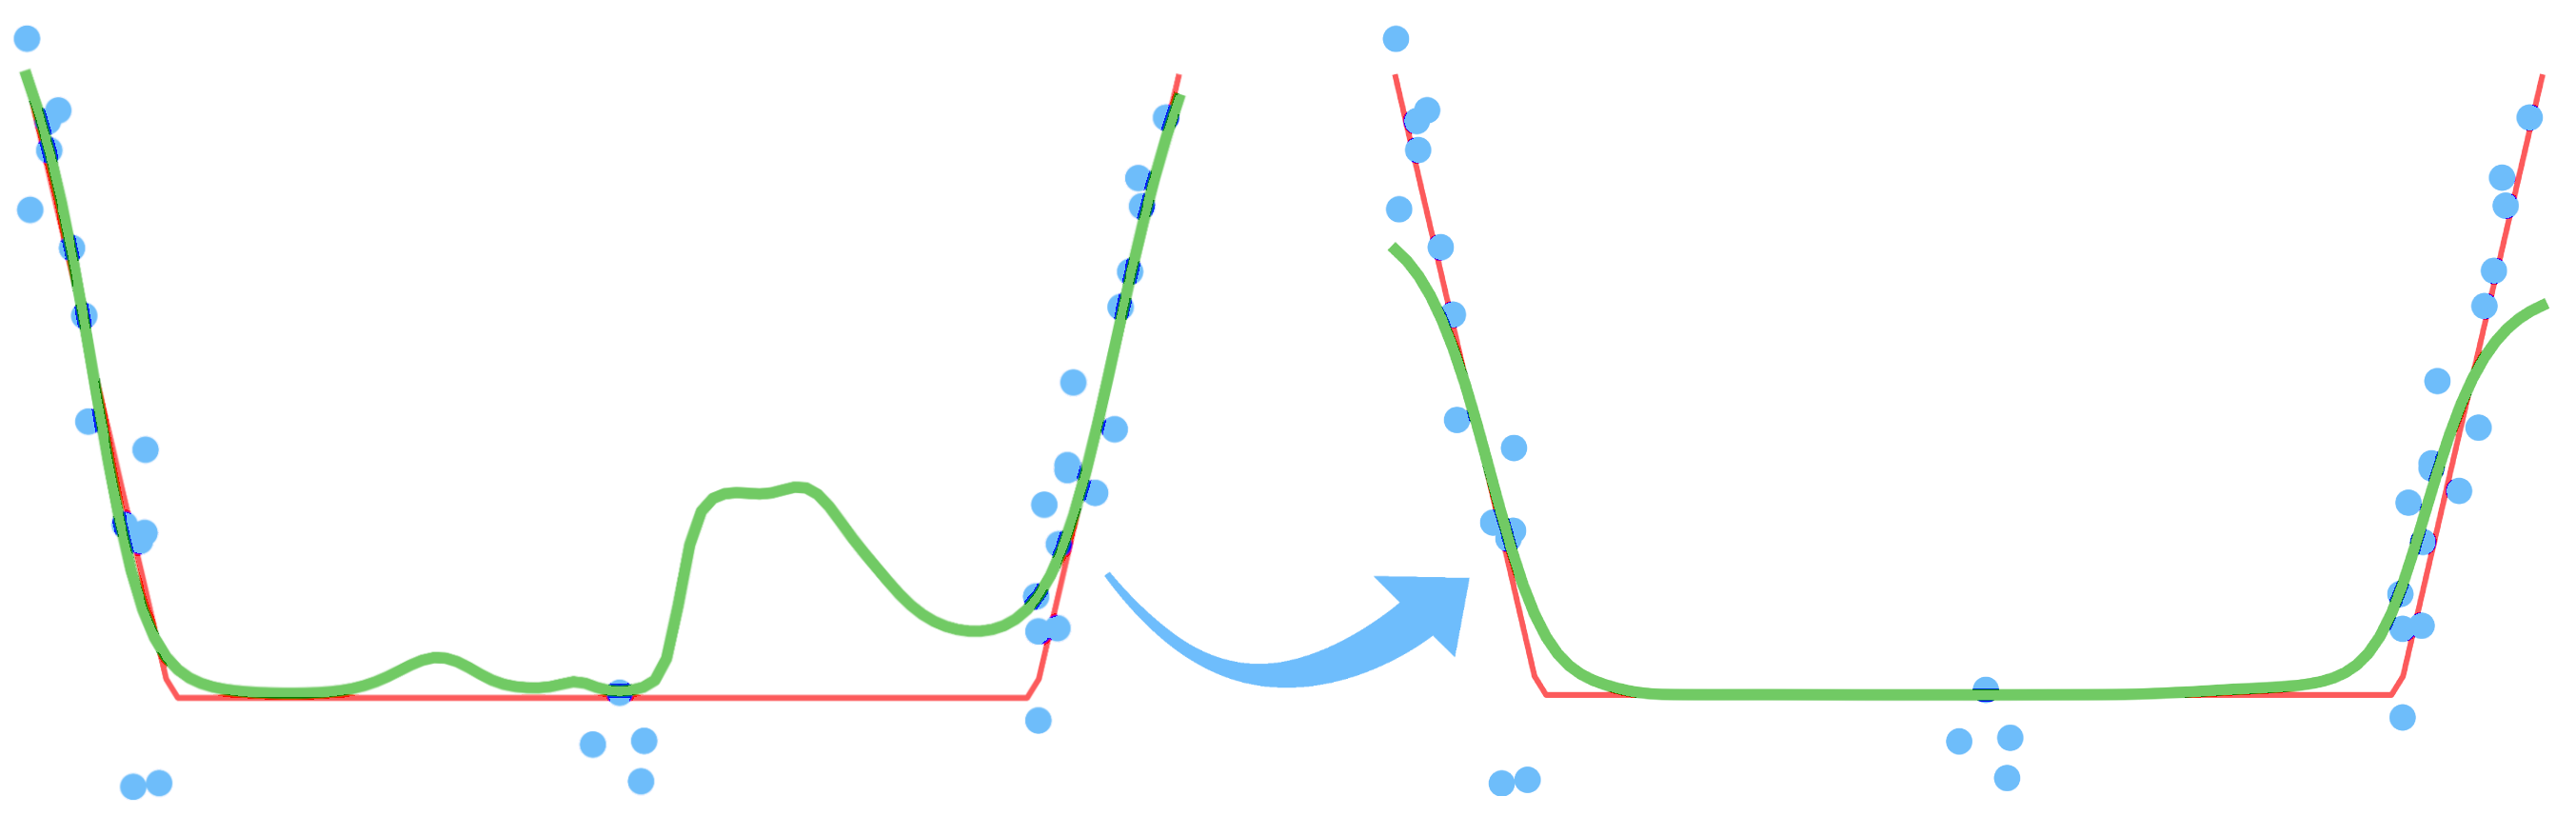
\includegraphics[width=.5\textwidth]{atelier/CLIP/CLIP.png}
\end{wrapfigure}
%
%
In the following we consider classification problems with $C\in\N$ different classes and functions $\net:\Inp\to\Delta^C$ for which we denote by 
\begin{align*}
\net^\MAP(\inp):=\argmax_c \net(\inp)_c
\end{align*}%
%
the maximum a posteriori estimation for input $\inp\in\Inp$. The capabilities of neural networks to perform classification tasks on unseen data---i.e. inputs $x\in\Inp$ that are not part of the training data---are impressive and the reason for their popularity. However, it has been noticed in \cite{goodfellow2014explaining} that is relatively easy to \enquote{fool} classification networks in the following sense:
%
\begin{center}
\textit{
Given a classification network and a human classifier $f_\param, h:\Inp\to\Delta^C$, and an input $\inp\in\Inp$ such that $f_\param^\MAP(\inp) = h^\MAP(\inp)$. An adversarial example is an input $\inpp\in \Inp$ that is close to $\inp$ and
%
\begin{align*}
f_\param(\inpp)\neq h(\inpp) = h(\inp).
\end{align*}
}
\end{center}
%
%
The vague concept of a \emph{human classifier}, bears the intuition of the classification problem as a human would solve it. Assuming that we are given data $\tset\subset \Inp\times\Oup$ that is samples i.i.d. from a joint distribution $P_{\Inp,\Oup}$ this function could also be chosen as $h(x)_c:=P_{\Inp,\Oup}(c|\inp)$.


\begin{remark}{}{}
While we mostly focus on neural networks, some authors argue that these instabilities are inherent to certain classification problems \cite{shafahi2018adversarial, fawzi2018adversarial}. From this point of view, trying to defend against these instabilities is not necessarily desirable.
\end{remark}
%
%
%
\paragraph{What are Adversarial Examples Formally} In order to formalize this idea we omit any influence of the typically unavailable function $h$ and instead consider $\inpp$ adversarial if $\net_\param(\inp)\neq\net_\param(\inpp)$, i.e. we assume $\net_\param(\inp)$ to be \enquote{correct}. Furthermore, in this work we assume that $\Inp$ models an image space $\Inp=\R^{K\times N\times M}$, with $K,N,M\in\N$ and choose a distance $d:\Inp\times\Inp\to\R^+_0$ to measure the distance between points in $\Inp$. 
%
\begin{remark}{}{}
In most of our examples we choose $d(\cdot,\cdot) = \norm{\cdot - \cdot}_p$. Employing a $L^p$ norm in an image context---via pixel-wise comparison---can be an unfavorable choice. Images that appear very different visually, (i.e. for a human classifier) can have a smaller $L^p$ distance, than images that visually appear similar, see e.g. \cite[Fig. 16]{stanczuk2021wasserstein}. However, it is easy tp evaluate, which is crucial for most applications. In the absence of a better criterion, having a small $L^p$ norm, is commonly the only way to decide if $\inpp$ is an admissible adversarial example. 
\end{remark}
%
%
\noindent%
Employing these simplifications we then say that $\inpp\in\Inp$ is adversarial, if
%
\begin{align*}
d(\inp,\inpp) \leq \budget \qquad \text{ and } \qquad \net_\param(\inp)\neq \net_\param(\inpp),
\end{align*}
%
where $\budget$ is called the \emph{adversarial budget}. This parameter
%
This interpretation only makes sense, if we assume that $\net_\param(\inp)$ is \emph{correct}, which can only be easily checked on the training data \cite{bungert2023begins}.
%
%
\paragraph{Types of Adversarial Examples} Typically, adversarial examples are created from the clean image $\inp$ via some distortion $\delta\in\R^n$. Together with an application map $T:\Inp\times\R^s\to\Inp$ one then obtains $\inpp=T(x,\delta)$ as the adversarial example. In this formulation one can the alternatively employ the criterion $\norm{\delta}\leq \budget$ to decide, whether $T(\inp,\delta)$ is an adversarial example. We only list some of the approaches below:
%
\begin{itemize}
\item\textbf{Addition}: the most well-known examples are created by $T(x,\delta):=\inp+\delta$, i.e. $\inpp = \inp + \delta$. Here, it is important to note that typically images are assumed to have values between $0$ and $1$, i.e. $\Inp=[0,1]^{K\times N\times M}$ for which it is important to ensure that $\inpp\in\Inp$.
%
\item\textbf{Translation and Rotation}: Simple geometric transformations---that would be unnoticeable for a human classifier---are quite effective to fool neural networks. Employing translations $T_{\text{t}}:\Inp\times\Inp\to\Inp$ one has to choose the behavior on the boundary such that one obtains a valid image. The same holds true for rotations $T_{\text{r}}:\Inp\times [-\pi,\pi]\to\Inp$. In this case $\delta\in[-\pi,\pi]$ models the angle of the rotation and would yield an admissible adversarial example, if $\abs{\delta}\leq \budget$. Here, we see that this formulation looses some expressivity:
%
\begin{itemize}
\item On the MNIST classification task, we see that only $\budget<\pi/2$ makes sense. Otherwise the number \enquote{6} could be always transformed to the number \enquote{9} and vice versa.
\item Considering the number \enquote{0} rotations above the angle $\pi/2$ can definitely yield proper adversarial examples $\inpp$.
\end{itemize}
%
We refer to \cite{engstrom2018rotation} for a study on these types of adversarial examples.
%
\item\textbf{Change of Basis}: As explored in \cite{guo2017countering} one can consider a different orthonormal basis of the image space $\R^{K\times N\times M}$ and then perform the attack w.r.t. this basis. 
The transform $T:\Inp\times\R^{K\times N\times M}\to\Inp$ first obtains the different representation of $\inp$, then adds the coefficients of $\delta$ and then maps back to the original basis. This is only meaningful, if one restricts certain coefficients of $\delta$ to be zero in the alternative basis. For example, the discrete cosine transform (\cite{ahmed1974discrete}) has been applied successfully in this context \cite{guo2017countering}.
\end{itemize}
%
%
In the following we restrict ourselves to the additive case and only consider examples $\inpp = \inp + \delta$.
%
%
\paragraph{Finding Adversarial Examples} Employing a loss function $\ell:\Oup\times\Oup\to\R$ the task of finding an adversarial examples $\inpp=\inp+\delta\in\Inp$ can be relaxed via solving the problem
%
\begin{align}\label{eq:advprob}
\max_{\inpp\in \Inp:d(\inp,\inpp)\leq \budget} \ell(\oup, \net_\param(\inpp))
=
\max_{\delta:\norm{\delta}_d\leq\delta, \inp+\delta\in\Inp}
\ell(\oup, \net_\param(\inp+\delta),
\end{align}
%
where $\oup=\net_\param(\inp)$. Solving this problem is referred to as \emph{attacking} the network $\net$. More precisely, this is a so-called \emph{untargeted} attacks, since we do not prescribe $\inpp$ to realize any special output as long as it confuses the network. Opposed to this, there are so called \emph{targeted} attacks. Here we pick $c^\adv \neq \net^\MAP_\param(\inp)$ and then want to find $\inpp$ such that $\net^\MAP_\param(\inpp) = c^\adv$. Here, we then consider the problem
%
\begin{align*}
\min_{\inpp\in \Inp:d(\inp,\inpp)\leq \budget} \ell(c^\adv_{\oh}, \net_\param(\inpp)).
\end{align*}
%
%
However, we see that conceptually this problem is similar to \cref{eq:advprob} and differs only by a change of sign and a different reference label.
%
A popular method to solve \cref{eq:advprob} is the projected sign gradient ascent iteration \cite{kurakin2016adversarial},
%
\begin{align*}
\inpp^\k{k+1} = \operatorname{Proj}_d(\inpp^\k{k} + \tau \sign(\nabla_{\inpp}
\ell(\net_\param(\inp), \net_\param(\inpp^\k{k})))).
\end{align*}
%
%
%
Here, $\operatorname{Proj}_d$ denotes the projection onto the set $\Inp\cap B_{d,\budget}(\inp)$, where $B_{d,\budget}(\inp)$ is the ball with radius $\budget$ around $\inp$, w.r.t. to the distance $d$. Performing only one step of this iteration yields the fast gradient sign method \cite{goodfellow2014explaining}. There is a wide variety of these so-called gradient-based white-box attacks \cite{yuan2019adversarial}, i.e. methods that assume that the gradient of the model is available. In more realistic scenarios, this might not be the case. Attacks that do not employ the actual gradient of the model to attack are called \emph{black box} attacks \cite{ilyas2018black}, which however not part of this thesis.
%
%
\paragraph{Defending Against Adversarial Examples}
%
%
We consider the question of finding parameters $\param\in\Param$ such that corresponding model $\net_\param$ is \emph{adversarially robust}, i.e. is less vulnerable to attacks. Therefore, we want the attack problem in \cref{eq:advprob} to be hard to solve. This intuition leads to the optimization problem
%
\begin{align*}
\min_{\param\in\Param} \sum_{(\inp,\oup)\in \tset} \max_{\inpp\in B_{d,\budget}(\inp)} \ell(\net_\param(\inpp), \oup)
\end{align*}
%
which is known as the \emph{adversarial training} formulation \cite{kurakin2016adversarial2, madry2017towards}. From a distributionally robust optimization point of view, this problem relates to 
%
\begin{align*}
\min_{\param\in\Param} \max_{\tilde P: D(P_{\Inp,\Oup}, \tilde P)\leq\budget} \int_{\Inp\times\Oup} \ell(\net_\param(\inp), \oup)\ d\tilde{P}(\inp,\oup)
\end{align*}
%
where $D$ denotes some distance on probability distributions, see \cite{bungert2023geometry}. Employing a batched gradient descent type iteration, one then has to solve a problem of the form \Cref{eq:advprob} in every step, which can be interpreted as a form of data augmentation \cite{lecun1995learning}. 
%
%
%
\paragraph{Lipschitz Training of Neural Networks}
%
Adversarial robustness is closely related to the Lipschitzness of a network $\net_\param$. Namely, for inputs $\inp,\inpp\in\Inp$ that are close, we also want the outputs of $\net_\param$ to be close. In other words we want to find a small constant $L>0$ such that
%
\begin{align*}
\norm{\net_\param(\inp) - \net_\param(\inpp)}_\Oup \leq L\ \norm{\inp-\inpp}_\Inp,
\end{align*}
%
where we typically employ an $L^p$ norm both $\norm{\cdot}_\Inp$ and $\norm{\cdot}_\Oup$.
%
The smallest constant fulfilling this inequality is the Lipschitz constant $\Lip(\net_\param)$. Having some control over this constant can therefore relate to being adversarially robust.
%
\begin{remark}{}{}
Apart from adversarial robustness, having an upper bound on the Lipschitz constant of a neural network is also important for other applications, see e.g. \cite{hasannasab2020parseval, arjovsky2017wasserstein}.
\end{remark}
%
%
We employ the Lipschitz constant as a regularizer and consider the problem
%
\begin{align}\label{eq:LipReg}
\min_\param \empLoss(\param) +\lambda\ \Lip(\net_\param)
\end{align}
%
for a parameter $\lambda$. Unfortunately, computing the Lipschitz constant of neural networks is a NP-hard problem \cite{scaman2018lipschitz} for which many works employ the estimate
%
\begin{align}\label{ineq:lip_weights}
\lip(\net_\param) \ \leq \ \prod_{l=1}^L  \lip(\Phi_l) \leq 
C_\sigma \prod_{l=1}^L \norm{W_l},
\end{align}
%
where here $\norm{W_l}$ denotes some matrix norm and $C_\sigma$ depends on the Lipschitz constants of the activation functions, see \cite{Anil2019,gouk2020regularisation, Krishnan2020, Roth2020}.
%
This inequality is not sharp and usually overestimates the Lipschitz constant, as we see in the following example taken from \cite{bungert2021clip}.
%
\begin{example}{}{}
We consider a feed-forward neural network $\net_\param:\R\to\R$ with one hidden layer,
%
\begin{align*}
\Phi_1(z) &:= \relu(W_1 z) :=\left(\max\{z, 0\}, \max\{-z, 0\}\right)^T,\qquad 
W_1:= (1,-1),\\
\Phi_2(z) &:= W_2 z := z_1 + z_2,\qquad W_2:=(1,1)^T,\\
\net_\param&:= \Phi_2\circ\Phi_1.
\end{align*}
%
For $\inp\in\R$ we have that 
%
\begin{align*}
\inp&\geq 0 \qquad\Rightarrow\Phi_1(\inp) = (\inp, 0)^T \qquad\Rightarrow \net_\param(\inp)=\inp,\\
\inp&\leq 0 \qquad\Rightarrow\Phi_1(\inp) = (0, -\inp)^T \qquad\Rightarrow \net_\param(\inp)=-\inp,
\end{align*}
%
and therefore $\net_\param = \abs{\cdot}$, for which we know that $\Lip(\net_\param)=1$. However employing the spectral for $W_1$ and $W_2$, we see that
%
\begin{align*}
\norm{W_1}\cdot\norm{W_2} = \sqrt{2}\ \sqrt{2} = 2.	
\end{align*}
%
\end{example}
%
Plugging the estimate of \cref{ineq:lip_weights} into \cref{eq:LipReg} therefore potentially over regularizes the problem.
%
\paragraph{Contribution in \cite{bungert2021clip}} In \cite{bungert2021clip} we propose a strategy to solve \cref{eq:LipReg} approximately, without the estimate in \cref{ineq:lip_weights}. The basic idea consists of approximating the Lipschitz constant on a finite set and using this approximation as a regularizer. Furthermore, we analyse the original model in \cref{eq:LipReg} where we study existence of solutions, the influence of the parameter $\lambda$ and the limits $\lambda\to 0, \lambda\to \infty$, see \cref{sec:CLIPAna}. Finally, we demonstrate the efficiency of the methods by applying to some simple toy problems, see \cref{sec:CLIPNum}.


\subsection{Cheap Lipschitz Training}
As mentioned before, we approximate the Lipschitz constant on a finite set $\Inp_{\lip{}}\subset\Inp\times\Inp$ via
%
\begin{align*}
\Lip(\net_\param; \Inp_{\lip{}}) := 
\max_{(\inp,\inpp)\in\Inp_{\lip{}}} \frac{\norm{\net_\param(\inp)-\net_\param(\inpp)}_\Oup}{\norm{\inp-\inpp}_\Inp}
\approx
\Lip(\net_\param).
\end{align*}
%
%
Disregarding the non-differentiable points of $\param\mapsto \Lip(\net_\param; \Inp_{\lip{}})$ allows us to make the above approximation in \cref{eq:LipReg} and the solve then problem via a gradient descent variant.
%
\begin{remark}{}{}
Let $f,g:\Inp\to\Oup$ be two differentiable functions. If $f(\inpp)>g(\inpp)$ for some $\inpp\in\Inp$ then we know that there exists some $\epsilon>0$ such that $f(\inp)>g(\inp)\forall \inp\in B_\epsilon(\inpp)$. We have that $f\vee g = \max\{f,g\} = f$ in $B_\epsilon(\inpp)$ and therefore $\inp\mapsto f(\inp)\vee g(\inp)$ is differentiable in $\inpp$. If $f(\inpp)=g(\inpp)$ then $f\vee g$ could be non-differentiable at $\inpp$. However, in practice we employ automatic differentiation, where in this case one of the functions is chosen, say $f$, and the \emph{gradient} at $\inpp$ is computed as $\nabla f$. 
\end{remark}
%
%
\noindent%
The strength of this approach of course is dependent on the quality of the set $\Inp_{\lip}$. In \cite{bungert2021clip} we propose to iteratively update the set via a gradient ascent type scheme. Namely, we initialize $\Inp_{\lip}$ as a random perturbation of a subset of the given data. In each step we then update the points as follows:
\begin{itemize}
\item Consider $L(\inp,\inpp) := {\norm{\net_\param(\inp)-\net_\param(\inpp)}}\,/\,{\norm{\inp-\inpp}},\quad\inp,\inpp\in\Inp$.
\item For each $(\inp,\inpp)\in\Inp_{\lip}$ perform the update 
%
\begin{align*}
\inp\phantom{'} &\gets \inp\phantom{'} + \tau\,L(\inp,\inpp) \nabla_{\inp} L(\inp,\inpp),\\
\inpp &\gets \inpp + \tau\,L(\inp,\inpp) \nabla_{\inpp} L(\inp,\inpp),
\end{align*}
%
for a parameter $\tau>0$.
\end{itemize}
%
This scheme performs a gradient ascent on the Lipschitz constant, see \cite[Alg. 1]{bungert2021clip}. For each mini batch $B\subset\tset$ we first update the set $\Inp_{\lip}$ and then update the parameters via
%
\begin{align*}
\param \gets \param - \eta\ \nabla_\param\left(\empLoss(\param; B) + 
\lambda~\Lip(\net_\param,\Inp_{\lip})\right)
\end{align*}
%
which yields the algorithm presented in \cite[Alg. 2]{bungert2021clip}. Similar to \cite{shafahi2019adversarial} one can reuse the gradients computed for $\nabla_\inp$ for the computation of $\nabla_\param$. This fact yields the attribute \emph{cheap} in the Lipschitz training algorithm.
%
\subsection{Analysis of Lipschitz Regularization}\label{sec:CLIPAna}
%
In \cite{bungert2021clip} we analyse some basic properties of the original regularization problem in \cref{eq:LipReg}. We repeat the assumptions we made therein, in order to refer to them in the following.

\begin{enumerate}[label= \textbf{Assumption \arabic*.}, ref={\arabic*}, align=left]
	\setlength{\itemsep}{9pt}
	\item\label[assumption]{ass:closs} We assume that the loss function 
	$\loss:\Oup\times\Oup\to\R\cup\{\infty\}$ satisfies:\\[-0.2cm]
	\begin{enumerate}
		\setlength{\itemsep}{6pt}
		\item $\loss(\oup,\oupp)\geq 0$ for all $\oup,\oupp\in\Oup$,
		\item $\oup\mapsto\loss(\oup,\oupp)$ is lower semi-continuous for all $\oupp\in\Oup$.
	\end{enumerate}
	% ###
	\item\label[assumption]{ass:net} We assume that the map $\param\mapsto\net_\param(\inp)$ 
	is continuous for all $\inp\in\Inp$.
	% ###
	\item\label[assumption]{ass:exist} We assume that there exists $\param\in\Param$ such that 
	\begin{align*}
		\frac{1}{\abs{\trSet}}
		\sum_{(\inp,\oup)\in\trSet}\loss(\net_\param(\inp),\oup)+
		\lambda \lip(\net_\param) < \infty.
	\end{align*}
\end{enumerate}
%
%
Employing only \cref{ass:net} one can show that that the map $\param\mapsto \Lip(\net_\param)$ is lower semi-continuous, \cite[Lem. 1]{bungert2021clip}. 
%
\paragraph{Existence} If $\Param$ is compact or finite, one can show that there exist solutions of \labelcref{eq:LipReg}. In the general case one needs to add a norm term, that ensures boundedness of a minimizing sequence. The following is the main existence result, which can be proven by the direct method in the calculus of variations \cite{dacorogna2007direct}.
%
\begin{proposition}{\cite[Prop. 1]{bungert2021clip}}{}
Under \cref{ass:closs,ass:net,ass:exist} the problem
\begin{align*}
\min_{\param\in\Param}
\frac{1}{\abs{\trSet}}
\sum_{(\inp,\oup)\in\trSet}
\loss(\net_\param(\inp),\oup) + 
\lambda\lip(\net_\param) + \mu\norm{\param}_\Param
\end{align*}
has a solution for all values $\lambda,\mu>0$.
Here, $\norm{\cdot}_\Param$ denotes a norm on $\Param$.
\end{proposition}
%
%
\paragraph{Dependency on the Regularization Parameter} Assuming that for every $\lambda>0$ we have a solution $\param_\lambda\in\Param$ of \cref{eq:LipReg} one can show that
%
\begin{alignat*}{2}
\lambda&\longmapsto
\frac{1}{\abs{\trSet}}
\sum_{(\inp,\oup)\in\trSet}\loss(\net_{\param_\lambda}(\inp),\oup) \quad&&\text{is non-decreasing,}
\\
\lambda&\longmapsto\lip(\net_{\param_{\lambda}}) 
\quad&&\text{is non-increasing.}
\end{alignat*}
%
%
This statement is the content of \cite[Prop. 2]{bungert2021clip}, however, the argument is exactly the same as in \cite{burger2013guide}. The intuition behind this result is that with increasing parameter $\lambda$ solutions of \cref{eq:LipReg}---more precisely the corresponding networks---have smaller Lipschitz constants, i.e. tend to be more constant, which however also diminishes their expressivity. We formalize the limit cases in the following.

Assuming the realizability condition of \cite{shalev2014understanding} we know that there exists parameters $\param\in\Param$ such that $\empLoss(\theta)=0$. This means there are parameters that fit the data perfectly. Considering the limit $\lambda\to 0$ we obtain convergence to a solution of the unregularized problem with the smallest Lipschitz constant.
%
\begin{proposition}{\cite[Prop. 3]{bungert2021clip}}{}
Let \cref{ass:closs,ass:net,ass:exist} and the realizability assumption~\cite{shalev2014understanding} be satisfied. If $\param_\lambda \to \param^\dagger\in\Param$ as $\lambda\searrow 0$, 
then
%
\begin{align*}
\param^\dagger\in\argmin\left\lbrace \lip(\net_\param) \st \param\in\Param,\, \frac{1}{\abs{\trSet}}
\sum_{(\inp,\oup)\in\trSet}\loss(\net_{\param}(\inp),\oup)
=0\right\rbrace
\end{align*}
%
if this problem admits a solution with $\lip(\net_\param)<\infty$.
\end{proposition}
%
%
\noindent%
Furthermore, we study the effect of sending $\lambda\to\infty$, where we see that the network $\net_{\param_\lambda}$ indeed tends to be constant as expected. We can explicitly characterize this constant as the closest point to barycenter of the output data, that is realizable by a neural network. 
%
\begin{proposition}{\cite[Prop. 4]{bungert2021clip}}{}
Let \cref{ass:closs,ass:net,ass:exist} be satisfied and assume that 
\begin{align*}
\mathcal{M}:=
\left\{\oup\in\Oup \st \exists\param\in\Param,\,
\net_\param(\inp)=y,\,\forall\inp\in\Inp\right\}\neq\emptyset.
\end{align*}
%
If $\param_\lambda \to \param_\infty \in\Param$ as $\lambda\to \infty$, then $\net_{\param_\infty}(\inp)=\hat{\oup}$ for all $\inp\in\Inp$ where 
\begin{align*}
\hat{\oup}\in\argmin_{\oup'\in\mathcal{M}}
\frac{1}{\abs{\trSet}}
\sum_{\oup\in\trSetY}\loss(\oup',\oup).
\end{align*}
\end{proposition} 
%
%
\clearpage%
\subsection{Numerical Results}\label{sec:CLIPNum}
%
 
\begin{wrapfigure}{r}{.4\textwidth}
\begin{center}

\includegraphics[width=.4\textwidth]{atelier/CLIP/CLIPQR.png}
\end{center}
The code for all the experiments is available at \href{https://github.com/TimRoith/CLIP}{github.com/TimRoith/}\\
\href{https://github.com/TimRoith/CLIP}{CLIP}.
\end{wrapfigure}
We briefly comment on the numerical results \cite{bungert2021clip}. All the experiments were implemented in \texttt{Python} \cite{van1995python} employing---among others---the \texttt{PyTorch} \cite{paszke2019pytorch} package. We conduct experiments on the MNIST \cite{leCun10} and FashionMNIST \cite{Han17} datasets.

\paragraph{Qualitative Example} We first apply the CLIP scheme to regularize a one-dimensional regression problem. In Fig.2 therein, one observes can observe qualitatively the effect of the regularization. Namely, we are given noisy data from a ground truth function for which the unregularized problem tend to overfit the data. The resulting network has fluctuations and therefore a large Lipschitz constant in certain regions, where the ground truth function has a small Lipschitz constant. With increasing parameter $\lambda$ we observe that the networks $f_{\param_\lambda}$ are smoothed out and better approximate the ground truth function.
%
\paragraph{Quantitative Evaluation of Adversarial Robustness} We additionally evaluate how robust a CLIP trained network is against adversarial attacks. Next to a standard learning rate scheduler, we also update the regularization parameter $\lambda$ throughout the training process. Namely, we choose a target accuracy be and evaluate the loss on a validation set after the epoch. If this accuracy is less then the target we decrease $\lambda$ and increase it if the accuracy is higher. In Table 1 of \cite{bungert2021clip} we compare ourselves against a weight regularization scheme that is based on the estimate in \cref{ineq:lip_weights}. We see that CLIP outperforms this method in most cases.
%
%
%
%
%
%
%
%
\clearpage%
\section{Sparsity via Bregman Iterations: \cite{bungert2022bregman}}\label{sec:BREG}
%
\begin{wrapfigure}{r}{.5\textwidth}
\centering
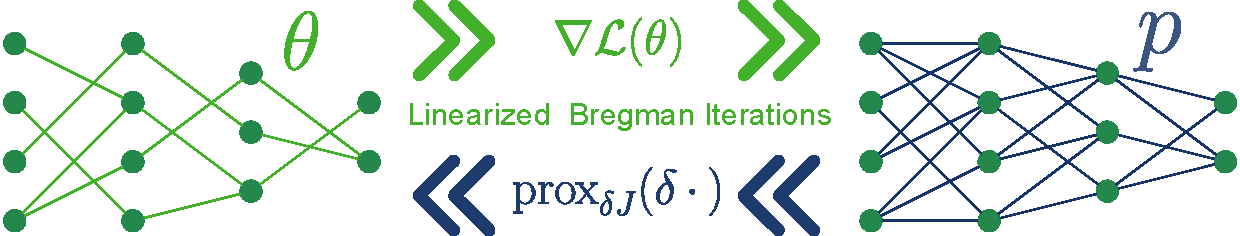
\includegraphics[width=.5\textwidth]{atelier/Breg_dist/BregmanPosterCartoon.pdf}
\end{wrapfigure}
%
%
Starting from the first simple neural architectures (e.g. \cite{rosenblatt1958perceptron}) the size of typical architectures has grown significantly in the last years \cite{hoefler2021sparsity}. While this development allowed to solve increasingly difficult tasks with neural networks, it also lead to immense computational requirements, both for the training and evaluation of the net. Therefore it seems natural, how the weights of neural networks can be compressed or more general how evaluation and training can be made more efficient. Some of the approaches here include (see \cite{gholami2021survey} for a comprehensive overview):
%
\begin{itemize}
\item \textbf{Architecture Optimization}: Designing an architecture that can be trained to have the same performance as a comparable one, while having less parameters, e.g. \cite{elsken2019neural, howard2017mobilenets}.
%
\item \textbf{Quantization}: Lowering the precision of the machine numbers of the parameters, e.g. \cite{banner2018scalable, courbariaux2014training}.
%
\item \textbf{Knowledge distillation}: Employing a trained larger network to learn a smaller network in a student-teacher approach, e.g. \cite{schmidhuber1992learning, hinton2015distilling}.
%
\item \textbf{Pruning}: Parameters with small saliency, i.e., parameters that contribute little to the effective output of the network are removed or set to zero, in order to obtain a sparse weight matrix or a smaller architecture, see e.g. \cite{lecun1989optimal, hassibi1993optimal}.
\end{itemize}
%
%
From the above methods, the pruning approach is most influential to our work in \cite{bungert2022bregman}. Namely, the concept of compressing the neural network by sparsifying the weight matrices is similarly employed. However, there are a few deviations from the classical pruning framework, which we remark in the following.

\paragraph{Sparsity via Optimization} In \cite{lecun1989optimal, hassibi1993optimal} one assumes to be given a trained neural network, which is then compressed after training based on some criterion. The authors in \cite{castellano1997iterative} employ an iterative pruning scheme, where a similar criterion is employed in order to throw away certain network weights after each step. In our work we want to employ a $L^1$ type penalty on weight matrices $W\in\R^{n\times m}$,
%
\begin{align*}
\norm{W}_1 = \sum_{i=1}^n\sum_{j=1}^m \abs{W_{ij}}
\end{align*}
%
which has been widely employed to obtain sparse solution, e.g. \cite{claerbout1973robust}. In \cite{tibshirani1996regression} this yields to the so-called Lasso problem
%
\begin{align*}
\min_\param \empLoss(\param) + \lambda \norm{\param}_1,\qquad \lambda >0,
\end{align*}
%
where we extend the $L^1$ norm to $\Param$ as discussed in \cref{sec:Bregnum}. This problem can for example by solved by a proximal gradient descent iteration
%
\begin{align}\label{eq:proxgd}
\param^\k{k+1} = \operatorname{soft\ shrinkage}(\param - \tau \nabla\empLoss(\param^\k{k}))
\end{align}
%
where the shrinkage operator from \cref{ex:softshrink}. This iteration was employed in \cite{nitanda2014stochastic, rosasco2014convergence, reddi2016proximal} to train sparse neural networks.
%
%
\paragraph{Sparse-to-Sparse Training} All of the sparsity-based methods mentioned before start with dense weight matrices and only decrease the number of parameters during or at the end of the training process. Our approach yields an iteration, where the network is sparse throughout the iteration. In fact we start with only very few non-zero parameters and only activate necessary weights during training. This paradigm is known as sparse-to-sparse or evolutionary training \cite{mocanu2018scalable, dettmers2019sparse, Evci2020, dai2019nest, fu2019exploring, huang2016split, liu2021}.
%
%
\paragraph{Contribution in \cite{bungert2022bregman}}
%
Our work falls into the regime of sparse-to-sparse training. However, instead of relying on some heuristic growth strategy, we employ the concept of inverse scale flows (see \cref{sec:convprelim}) which allows us to obtain a optimization-driven framework, with a time-continuous interpretation. We propose a stochastic variant of linearized Bregman iterations (\cref{sec:Bregmom}) and employ it to train a sparse neural network. We show monotonic decrease of the loss in the stochastic setting---which is not possible in the case of proximal gradient descent \cref{eq:proxgd}---and convergence of the iterates under additional convexity assumptions, see \cref{sec:ConvAna}. Finally, we demonstrate the numerical efficiency of the method (see \cref{sec:Bregnum}) and provide an interesting applications for neural architecture search, which was further developed in \cite{bungert2021neural}.


\subsection{Preliminaries on Convex Analysis and Bregman Iterations}\label{sec:convprelim}

We first review some necessary concepts from convex analysis that allow us to introduce the framework in \cite{bungert2022bregman}. We refer to \cite{benning2018modern, rockafellar1997convex, bauschke2011convex} for a more exhaustive introduction to the topics.
%
The functional $\func$ is called lower semicontinuous if $\func(u)\leq\liminf_{n\to\infty}\func(u_n)$ holds for all sequences $(u_n)_{n\in\N}\subset\Param$ converging to $u$.
%
\begin{definition}{}{}
Given a Hilbert space $\Param$ and a functional $\func:\Param\to(-\infty,\infty]$.
%
\begin{enumerate}
\item The functional $\func$ is called convex, if
%
\begin{align}
    \func(\lambda\overline{\param}+(1-\lambda)\param)\leq
    \lambda\func(\overline{\param})
    +(1-\lambda)\func(\param),\quad\forall\lambda\in[0,1],\,\overline{\param},\param\in\Param.
\end{align}
%
\item The effective domain of $\func$ is defined as $\dom(\func):=\{\param\in\Param\st\func(\param)\neq\infty\}$ and $\func$ is called proper if $\dom(\func)\neq\emptyset$.
\end{enumerate} 
\end{definition}
%
%
In the following we want to consider functionals $J$ that are convex, but not necessarily differentiable. Therefor, we define the subdifferential.
%
\begin{definition}{}{}
of a convex {and proper} functional $\func:\Param\to(-\infty,\infty]$ at a point $\param\in\Param$ as
% ---------------------------------------------------------
\begin{align}
\label{eq:subgrad}
    \partial\func(\param) := \left\lbrace \sg\in\Param \st \func(\param) + \langle\sg,\overline{\param}-\param \rangle \leq \func(\overline{\param}),\;\forall\overline{\param}\in\Param\right\rbrace.
\end{align}
\end{definition}
% ---------------------------------------------------------
If $\func$ is differentiable, then the subdifferntial coincides with the classical gradient (or Fr\'echet derivative). We denote $\dom(\partial\func):=\{\param\in\Param\st\partial\func(\param)\neq\emptyset\}$ and observe that $\dom(\partial\func)\subset\dom(\func)$.

The main algorithm in this section are so-called Bregman iterations, for which we first define the Bregman distance.
%
\begin{definition}{Bregman Distance}{}
Let $\func:\Param\to(-\infty,\infty]$ be a proper, convex functional. Then we define for $\param\in\dom(\partial\func),\overline{\param}\in\Param$
% ---------------------------------------------------------
\begin{align}\label{eq:bregman_distance}
D^\sg_\func(\overline{\param},\param) := \func(\overline \param)-\func({\param})-\langle\sg,\overline\param-{\param}\rangle,\quad\sg\in\partial\func(\param).
\end{align}
%
For $\sg\in\partial\func({\param})$ and $\overline\sg\in\partial\func(\overline{\param})$ we define the \emph{symmetric} Bregman distance as
\begin{align}
D^\mathrm{sym}_\func(\overline{\param},\param) := D^\sg_\func(\overline{\param},\param) + D^{\overline{\sg}}_\func(\param,\overline\param).
\end{align}
\end{definition}
% ---------------------------------------------------------
Intuitively, the Bregman distance $D^\sg_\func(\overline{\param},\param)$, measures the distance of $\func$ to its linearization around $\param$, see \cref{fig:Bregdist}. If $J$ is differentiable, then the subdifferential is single valued---we can suppress the sup script $\sg$---and we have
%
\begin{align*}
D_J(\overline\param,\param) = \func(\overline \param)-\func({\param})-\langle\,\nabla \func(\param), \overline\param-{\param}\rangle.
\end{align*}
%
\begin{figure}
\centering
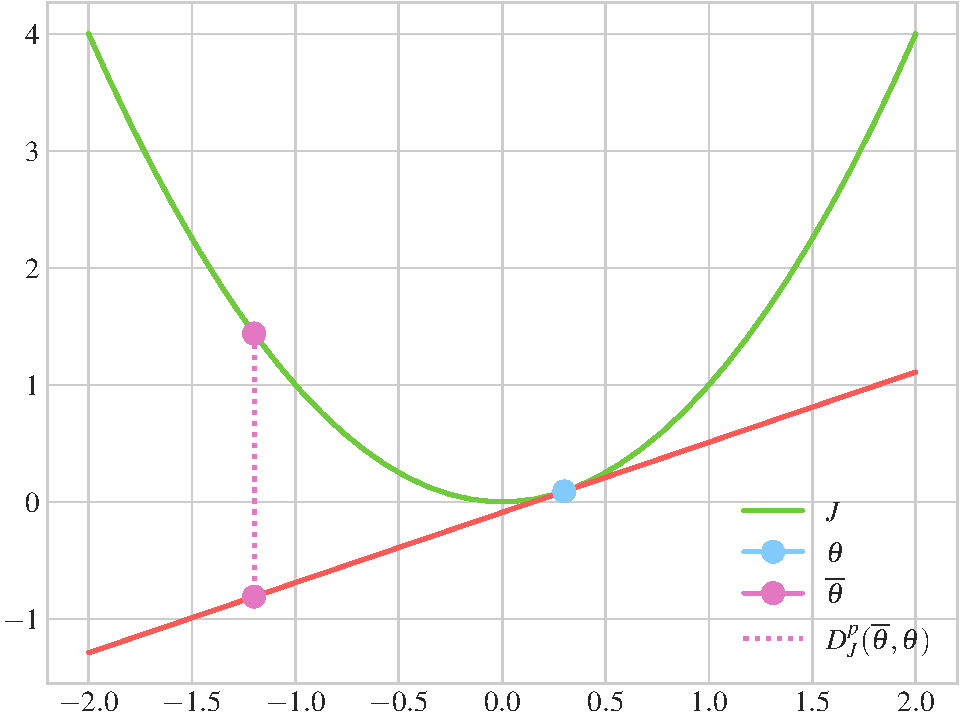
\includegraphics[width=.7\textwidth]{code/Bregman/lin_dist.pdf}
\caption{Visualization of the Bregman distance.}\label{fig:Bregdist}
\end{figure}
%
\begin{example}{}{ex:BregNorm}
For $\Param=\R^n$ and $J=\frac{1}{2}\norm{\cdot}_2^2$ we see that $\partial J(\param) = \{\param\}$ and therefore
%
\begin{align*}
D_J^p(\overline{\param}, \param) &= 
\frac{1}{2}\langle \overline\param,\overline\param\rangle - 
\frac{1}{2}\langle \param,\param\rangle - \langle \param, \overline\param-\param\rangle 
\\&=
\frac{1}{2}\langle \overline\param,\overline\param\rangle+
\frac{1}{2}\langle \param,\param\rangle -
\langle \param,\overline\param\rangle
\\&=
\frac{1}{2}\norm{\overline\param - \param}_2^2 = J(\overline\param - \param).
\end{align*}
\end{example}
%
We can easily see that in general it is neither definite, symmetric nor fulfills the triangle inequality, hence it is not a metric. 
However, it fulfills the two distance axioms
\begin{align}
D^\sg_\func(\overline{\param},\param) \geq 0,\quad D^\sg_\func(\param,\param)=0,\quad\forall\overline{\param}\in\Param,\param\in\dom(\partial\func).
\end{align}
%
The same holds for the symmetric Bregman distance, where additionally---as the name suggests---the symmetry property is fulfilled.
%
%
The last concept that is crucial in \cite{bungert2022bregman} is the so-called proximal operator.
%
\begin{definition}{}{}
Let $\func:\Param\to(-\infty,\infty]$  be convex, proper and lower semicontinuous functional, then we define the \emph{proximal operator} as
\begin{align*}
    \prox{\func}(\overline{\param}) := \argmin_{\param\in\Param} \frac{1}{2}\norm{\param-\overline{\param}}^2 + \func(\param).
\end{align*}
\end{definition}
%
If $\func$ is additionally a closed function, i.e., its sublevel sets
%
\begin{align*}
N_\alpha = \{\param\in\dom \func: \func(\param)\leq \param\}
\end{align*} 
%
are closed for every $\alpha\in\R$ then we have that the function $\tilde J = \frac{1}{2}\norm{\param -\cdot}^2 + \func(\param)$ is closed, proper and \emph{strongly} convex and therefore has a unique minimizer, see \cite[Thm. 27.1]{rockafellar1997convex}. Additionally, one often considers a regularization parameter $\lambda>0$ and is then interested in $\prox{\lambda \func}$.
%
\begin{remark}{}{}
The the optimality conditions for $\param=\prox{\lambda J}(\overline\param)$ yield 
%
\begin{align*}
\pparam - \param \in \lambda \partial \func(\param).%
\end{align*}
%
For a proper, closed and convex function we obtain
%
\begin{align*}
\param = (I + \lambda\partial\func)^{-1}(\pparam)
\end{align*}
%
where $(I + \lambda\partial\func)^{-1}$ is called the \emph{resolvent} and is a one-to-one mapping (see \cite[Ch. 3.2]{parikh2014proximal})  which justifies the equality in the above equation. If $\func$ is differentiable, then we have $\partial \func = \{\nabla \func\}$ and therefore,
%
\begin{align*}
\prox{\lambda\func} = (I + \lambda\nabla\func)^{-1}.
\end{align*}
\end{remark}
%
%
\noindent%
In the following we list two relevant examples for the application in \cite{bungert2022bregman, bungert2021neural}.
%
\begin{example}{}{ex:softshrink}
If $\func=\norm\cdot$ is a norm and $\lambda>0$ then we have that (see e.g. \cite{parikh2014proximal})
%
\begin{align*}
\prox{\lambda\func}(\pparam) = 
\pparam - \operatorname{Proj}_{\norm{\cdot}^\ast}(\pparam/\lambda)
\end{align*}
%
where $\operatorname{Proj}_{\norm{\cdot}^\ast}$ denotes the projection operator w.r.t. the dual norm $\norm{\param}^\ast = \sup\{\abs{\langle f , \param\rangle}: f\in\Theta^\ast\}$. In the case of $\ell^p$ norms on $\R^n$ we know that that 
%
\begin{align*}
\norm{\param}_p^\ast = \norm{\param}_q
\end{align*}
%
with $1/p + 1/q = 1$ with the notational convention of $1/\infty=0$. Especially relevant are the cases $p\in\{1,2\}$. Here, we then have that
%
\begin{align*}
\prox{\lambda\norm{\cdot}_2}(\pparam) = 
%
\pparam\,\left(1 - \min\left\{\frac{\lambda}{\norm{\pparam}_2}, 1\right\}\right)=
%
\begin{cases}
\pparam\,(1 - \lambda/\norm{\pparam}_2) &\text{ if } \norm{\pparam}_2 \geq \lambda\\
0 &\text{ else}
\end{cases}
\end{align*}
%
and for $i=1,\ldots,n$
%
\begin{align*}
\prox{\lambda\norm{\cdot}_1}(\pparam)_i
%
= \sign(\pparam_i)\, \max\left\{\abs{\pparam_i} - \lambda, 0\right\} =
%
\begin{cases}
\pparam_i -\lambda &\text{ if }\pparam > \lambda\\
0 &\text{ if } \abs{\pparam_i}\leq \lambda\\
\pparam_i +\lambda &\text{ if }\pparam < -\lambda
\end{cases}
\end{align*}
%
the so called \emph{soft shrinkage operator}. 
\end{example}
%
%
\begin{example}{Group Norms}{}
Another relevant functional $\func$ is the group norm $\ell_{1,2}$ that---in the context of sparse neural networks---was first employed by \cite{scardapane2017group}. Here, we assume that the parameters in $\Theta$ can be grouped in a collection of parameters $\mathcal{G}$, for which we the choose
%
\begin{align*}
\func(\param) = \sum_{g\in\mathcal{G}} \sqrt{\# \mathcal{G}} \norm{g}_2
\end{align*}
%
In this case the proximal operator is given as
%
\begin{align*}
\prox{\lambda\func}(\pparam)_g = g \, 
\max\left\{1- \min\left\{
\frac{\lambda\,\sqrt{\# \mathcal{G}}}{\norm{g}_2}
,1 \right\}
,0\right\}
\end{align*}
\end{example}
%
%
%\begin{example}{Elastic Net}{}
%For a convex functional $\func$ we also consider the elastic net version $J_\delta = J + \frac{1}{2\delta}\norm{\cdot}^2$ in the following. Here we see that 
%%
%\begin{align*}
%\prox{\lambda\func_\delta}(\pparam) &= \argmin_{\param\in\Param} \frac{1}{2}\norm{\param-\overline{\param}}^2 + \lambda\func(\param) + \frac{1}{2\delta}\norm{\param}^2\\ 
%%
%&= 
%\argmin_{\param\in\Param} \frac{1+\delta}{2\delta} \norm{\param}^2 - \frac{1}{2}\langle \param,\pparam\rangle + \lambda\func(\param)\\
%%
%&= \argmin_{\param\in\Param} \frac{1}{2} \norm{\param}^2 - \frac{1}{2}
%\left\langle \param,\frac{\delta}{1+\delta}\, \pparam\right\rangle + (1 + \delta)^{-1}\lambda J(\param)\\
%&= 
%\prox{\frac{\delta}{1+\delta}\lambda \func}\left(\frac{\delta}{1+\delta}\, \pparam\right).
%\end{align*}
%%
%Setting $\tilde\delta = \delta(1+\delta)^{-1}$ we see that for $\func = \norm{\cdot}_1$ we have that
%%
%\begin{align*}
%\prox{\lambda\func_\delta}(\pparam)_i = \sign(\tilde\delta\, \pparam_i) 
%\max\left\{
%\abs{\tilde\delta\,  \pparam_i} - \lambda, 0
%\right\}
%=
%\sign(\pparam_i)
%\end{align*}
%\end{example}
%
%
%
%
\paragraph{Bregman Iterations} Our goal is to minimize a function $\empLoss$ while simultaneously obtaining a low value w.r.t. the functional $J$. One popular approach considers the regularized problem
%
\begin{align*}
\min_\param \empLoss(\param) + \lambda \func(\param)\qquad \lambda>0,
\end{align*}
%
see e.g. \cite{tikhonov1943stability, combettes2008proximal,daubechies2004iterative,fadili2006sparse,figueiredo2007gradient,chambolle2004algorithm,chambolle2011first}, which however influences the minimizers of the original problem $\min_\param \empLoss(\param)$. In the derivation of the Bregman iterations one can take a different viewpoint. Assume that we want to employ an iterative scheme, where in each step we want minimize $\empLoss$ while penalizing the distance to the previous iterate. For a stepping parameter $\tau$ and starting from some $\param^\k0\in\Param$ this yields the update
%
\begin{align}\label{eq:minmom}
\param^\k{k+1} = \argmin_\param \tau\empLoss(\param) + \frac{1}{2}\norm{\param -\param^\k{k}}^2 
= \prox{\tau\empLoss}(\param^\k{k}).
\end{align}
%
At first sight this is either known as the proximal point algorithm \cite{bregman1967relaxation} or a minimizing movement scheme \cite{de1993new}. If $\empLoss$ is differentiable, this update can be rewritten as 
%
\begin{align*}
\param^\k{k+1} = (I+\tau\nabla\empLoss)^{-1}\param^\k{k}
%
\Leftrightarrow
%
\frac{1}{\tau}\left(\param^\k{k+1} - \param^\k{k}\right)
= -\nabla\empLoss(\param^\k{k+1})
\end{align*}
%
which is a implicit Euler discretization (\cite{euler1824institutionum}) of the time-continuos gradient flow
%
\begin{align*}
\partial_t \param_t = -\nabla\empLoss(\param_t).
\end{align*}
%
%
We see that the penalization term in \cref{eq:minmom} is in fact the Bregman distance of the functional $\frac{1}{2}\norm{\cdot}^2$. In order to incorporate an arbitrary convex functional $\func$---and therefore allow each iterate to only slightly deviate w.r.t. the Bregman distance of $\func$ to the previous iterate---we employ $D_\func^{\sg^\k{k}}(\cdot, \param^\k{k})$ as a penalization term. In order to obtain a update scheme for the subgradients, we observe
%
\begin{gather}
\param = \argmin_{\param\in\Param} D^{\sg^{(k)}}_\func\left(\param,\param^{(k)}\right) + \tau^{}\empLoss(\param)
\\
\Leftrightarrow
\sg^\k{k} + \tau\nabla\empLoss(\param)\in \partial\func(\param). 
\end{gather}
%
This finally yields \emph{Bregman iteration} of \cite{osher2005iterative}
%
%
\begin{subequations}\label{eq:bregman_iteration}
\begin{align}
\param^{(k+1)} &= \argmin_{\param\in\Param} D^{\sg^{(k)}}_\func\left(\param,\param^{(k)}\right) + \tau^{}\empLoss(\param), \\
\sg^{(k+1)} &= \sg^{(k)} - \tau^{}\nabla\empLoss(\param^{(k+1)}) \in \partial \func(\param^{(k+1)}).
\end{align}
\end{subequations}
%
The very nature of Bregman iterations means starting with a iterate $\param^{(0)}$ that has a low value in $J$---preferably $J(\param^{(0)}) = 0$---and only increase $J(\param^{(k)})$ gradually as $k$ increases.
%
\begin{remark}{}{}
Originally, the iterations were employed for solving inverse problems. Here, we are given a forward operator $A:\Param\to\tilde{\Param}$ and a noisy measurement $f= A\param +\delta$ where $\delta\in \tilde{\Param}$ is additive noise. The loss function is then of the form
%
\begin{align*}
\empLoss = \frac{1}{2}\norm{A\cdot - f}^2_2
\end{align*}
%
for which one can show that the Bregman iterations converge to a solution of
%
\begin{align}\label{eq:Bregexact}
\min \left\{\func(\param): A\theta = f\right\},
\end{align}
%
see e.g. \cite{osher2005iterative}. In comparison the concept of adding a regularizing term with parameter $\lambda>0$, i.e. considering the problem
%
\begin{align*}
\min_\param \empLoss(\param) + \lambda J(\param) 
\end{align*}
%
actually modifies the minimizers. In this sense Bregman iterations do not introduce a bias.
\end{remark}
%
%
\begin{example}{}{ex:BregCat}
In order to get an intuition about the behavior of Bregman iterations, we consider an image denoising task. I.e. we are given a noisy image $\R^{n\times m}\ni f = u + \delta$ where $\delta\in\R^{n\times m}$ is additive noise. In order to obtain $u\in\R^{n\times n}$ from $f$ we employ the TV functional \cite{rudin1992nonlinear} 
%
\begin{align*}
J(u) = TV(u) := \sum_{i,j} \sqrt{\abs{u_{i+1, j} - u_{i,j}}^2 + \abs{u_{i,j+1} - u_{i,j}}^2}
\end{align*}
%
together with the loss function $\empLoss(u):= \frac{1}{2}\norm{u-f}^2_2$.
%
We start with an image $u^{(0)}$ such that $TV(u^{(0)})=0$, i.e. a constant image. In \cref{fig:BregCat} we visualize the iteration. At lower iterations $u^{(k)}$ only displays features on a larger scale, while at the end, the iteration converges back to smallest possible scale, the noisy data. In order to obtain an appropriate denoising, one needs to employ a early stopping here. This fits well to the insight from \cref{eq:Bregexact} since here the forward operator is the identity, i.e.
%
\begin{align*}
\left\{ u: \frac{1}{2}\norm{u-f}^2=0\right\} = \{f\}. 
\end{align*}
%
It should also be noted that this example only serves a explanatory purpose. In practice directly applying \cref{eq:bregman_iteration} for $J=TV$ can become infeasible since the first minimization problem is expensive.
\end{example}%
%
%
%
%
\begin{figure}
\begin{minipage}{\textwidth}%
\begin{subfigure}{.3\textwidth}%
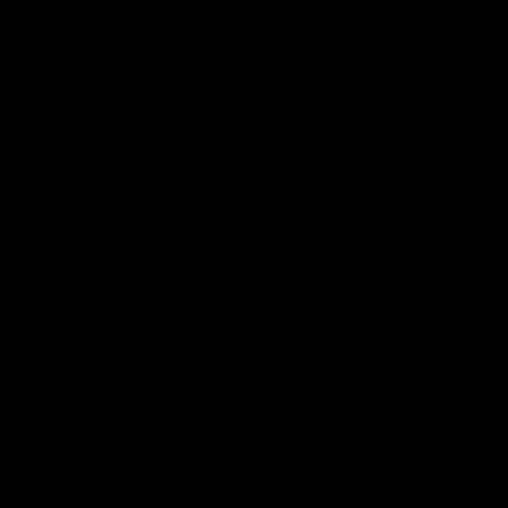
\includegraphics[width=\textwidth]{atelier/breg_cat/cat-0.png}
\subcaption{Iteration $k=0$}
\end{subfigure}\hfill%
\begin{subfigure}{.3\textwidth}%
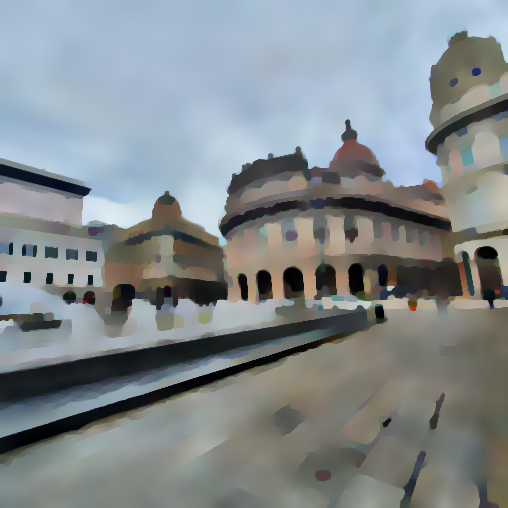
\includegraphics[width=\textwidth]{atelier/breg_cat/cat-10.png}
\subcaption{Iteration $k=10$}
\end{subfigure}\hfill%
\begin{subfigure}{.3\textwidth}%
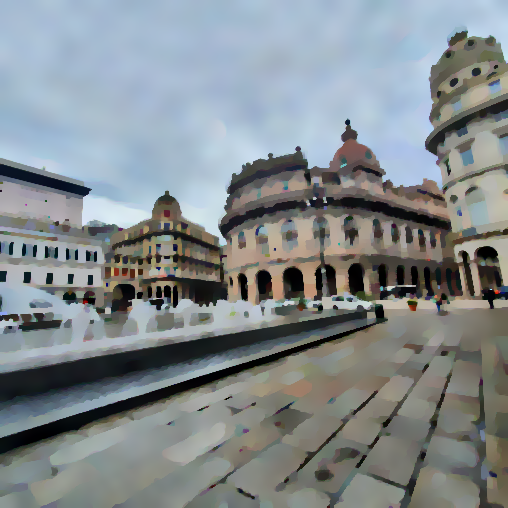
\includegraphics[width=\textwidth]{atelier/breg_cat/cat-20.png}
\subcaption{Iteration $k=20$}%
\end{subfigure}
\end{minipage}\\%

\begin{minipage}{\textwidth}%
\begin{subfigure}{.3\textwidth}%
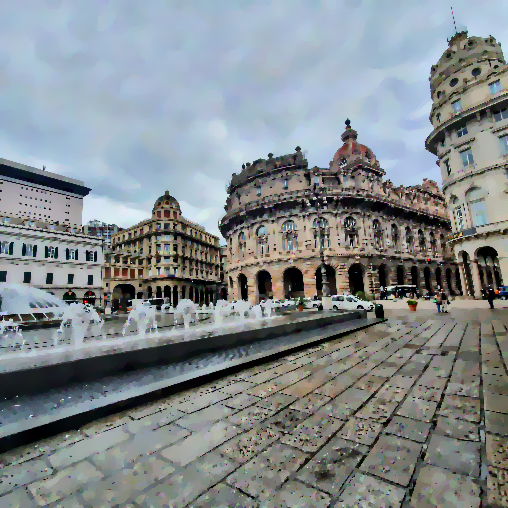
\includegraphics[width=\textwidth]{atelier/breg_cat/cat-50.png}%
\subcaption{Iteration $k=50$}%
\end{subfigure}\hfill%
\begin{subfigure}{.3\textwidth}%
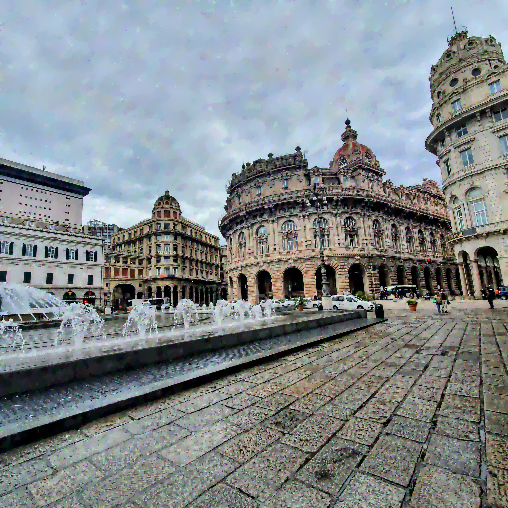
\includegraphics[width=\textwidth]{atelier/breg_cat/cat-95.png}%
\subcaption{Iteration $k=100$}%
\end{subfigure}\hfill%
\begin{subfigure}{.3\textwidth}%
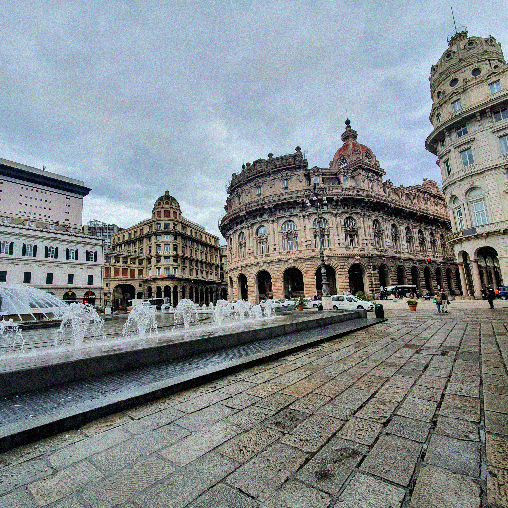
\includegraphics[width=\textwidth]{atelier/breg_cat/data.png}
\subcaption{Iteration $k=500$}
\end{subfigure}%
\end{minipage}%
%
\caption{Bregman iterations for image denoising in \cref{ex:BregCat}}\label{fig:BregCat}
\end{figure}%
%
%
\noindent
If $J=\frac{1}{2}\norm{\cdot}_2^2$ as in \cref{ex:BregNorm} then this amounts to the step
%
\begin{align*}
\param^{(k+1)} &= \argmin_{\param\in\Param} \frac{1}{2}\norm{\param - \param^{(k)}}^2_2 + \tau^{}\empLoss(\param),
\end{align*}
%
where the optimality conditions then yield
%
\begin{align*}
\param^{(k+1)} - \param^{(k)} + \tau \nabla \empLoss(\param^{(k+1)}) = 0
\Leftrightarrow \param^{(k+1)}= \param^{(k)} - \tau \nabla \empLoss(\param^{(k+1)})
\end{align*}
%
which is a standard implicit Euler iteration. The time continuous flow for $\tau\to 0$ is known as the \emph{inverse scale space} flow \cite{burger2006nonlinear,burger2007inverse},
%
\begin{align*}
\begin{cases}
    \dot{\sg}_t = - \nabla\empLoss(\param_t), \\
    \sg_t \in \partial \func(\param_t),
\end{cases}
\end{align*}
%
where again for $J=\frac{1}{2}\norm{\cdot}_2^2$ we obtain that $\partial J(\param_t) = \param_t$ and therefore obtain the standard gradient flow. Hence we see, that the inverse scale space flow is a generalization of the standard gradient flow. 
%
%
%
\subsection{Linearized Bregman Iterations and Mirror Descent}
%
The minimization step in \cref{eq:bregman_iteration} is infeasible for large scale applications, especially in our setting of neural networks. Therefore, we employ the idea introduced in \cite{yin2008bregman, cai2009convergence}. Here, we first linearize the loss function around the previous iterate,
%
\begin{align*}
\empLoss(\param) \approx \empLoss(\param^{(k)}) + 
\left\langle \nabla\empLoss(\param^{(k)}), \param - \param^{(k)}
\right\rangle.
\end{align*} 
%
The next step is to replace $\func$ with the strongly convex elastic net regularization%
\begin{align}\label{eq:elastic_net}
\func_\delta:= \func + \frac{1}{2\delta}\norm{\cdot}^2_2.
\end{align}
%
The minimization step then transforms to
%
\begin{align}\label{eq:LinBregDer}
\argmin_{\param\in\Param} &D^{\sg^{(k)}}_{\func_\delta} \left(\param,\param^{(k)}\right) + \tau^{}\left\langle \nabla\empLoss(\param^{(k)}), \param
\right\rangle\\&= 
\argmin_{\param\in\Param}
J(\param) + \frac{1}{2\delta} \norm{\param}^{2}_2 - 
\langle \sg^{k}, \param\rangle +
\tau^{}\left\langle \nabla\empLoss(\param^{(k)}), \param
\right\rangle\nonumber\\
&=
\argmin_{\param\in\Param}
J(\param) + \frac{1}{2\delta} \norm{\param - \delta(\sg^{(k)} -\tau \nabla\empLoss(\param^{(k)})}^2_2 - \underbrace{\norm{\sg^{(k)} -\tau \nabla\empLoss(\param^{(k)})}^2_2}_{\text{constant in } \param}\nonumber\\
&=
\prox{\delta \func}\left(\delta\left(\sg^{(k)} -\tau \nabla\empLoss(\param^{(k)}\right)\right).\nonumber%
\end{align}
%
Note that here $\sg^{(k)}$ is a subgradient of $J_\delta$ at $\param$ therefore we derive the subgradient update rule
%
\begin{align*}
\sg^{(k+1)} := \sg^{(k)} - \tau \empLoss(\param^{(k)}).
\end{align*}
%
This finally yields the linearized Bregman iterations
%
\begin{subequations}\label{eq:lin_bregman_iteration}
\begin{align}
\sg^{(k+1)} = \sg^{(k)} - \tau \nabla\empLoss(\param^{(k)}),\\
\param^{(k+1)} = \prox{\delta J}(\delta \sg^{(k+1)}).
\end{align}
\end{subequations}
%
%
The last line is equivalent to $\sg^{(k+1)}\in\partial J_\delta(\param^{(k+1)})$ for which we obtain the continuous linearized flow
%
\begin{align*}
\dot{\sg}_t &= -\nabla \empLoss(\param_t),\\
\sg_t &\in \partial J_\delta(\param_t),
\end{align*}
%
see \cite{burger2006nonlinear,burger2007inverse}.
%
%
\paragraph{Connections To Mirror Descent}
As already noticed by \cite{villa2023implicit} linearized Bregman iteration are equivalent to mirror descent in some situations. We show the equivalence in the following, where we employ similar arguments as in \cite{beck2003mirror}.
%
One assumes to be given a differentiable and strongly convex function $h:\Param\to\R$, i.e.,
%
\begin{align*}
h(\overline\param) - h(\param) - \langle\nabla h(\param), \overline\param - \param \rangle \geq  
\frac{1}{2} \norm{\overline\param - \param}^2_2
\end{align*}
%
for all $\param,\overline\param\in\Param$. The mirror descent update then reads (\cite{nemirovskij1983problem, beck2003mirror})
%
\begin{align}\label{eq:mirror}
\theta^{(k+1)} = \nabla h^\ast\left(\nabla h\left(\theta^{(k)}\right) - \tau \empLoss(\param^{(k)})\right)
\end{align}
%
where $h^\ast$ denotes the Fenchel conjugate
%
\begin{align*}
h^\ast(\sg) = \sup_{\param} \langle \sg, \param\rangle - h(\param)
\end{align*}
%
with the gradient (see \cite{boyd2004convex})
%
\begin{align*}
\nabla h^\ast(\sg) = \argmax_{\param} \left\{ \langle\sg, \param\rangle - h(\param)\rangle\right\}.
\end{align*}
%
Therefore, we see that \cref{eq:mirror} can be written as
%
\begin{align*}
\param^{(k+1)} &= \argmax_\param
\left\{\left\langle\nabla h\left(\theta^{(k)}\right) - \tau \empLoss(\param^{(k)}), \param \right\rangle - h(\param)\right\}\\
&=
\argmax_\param \left\{-D_h(\param, \param^{(k)})-\tau\left\langle \empLoss(\param^{(k)}), \param \right\rangle\right\}\\
&=
\argmin_\param \left\{D_h(\param, \param^{(k)})+\tau\left\langle \empLoss(\param^{(k)}), \param \right\rangle\right\}
\end{align*}
%
which was our starting point to derive linearized Bregman iterations for $h=\func_{\delta}$ in \cref{eq:LinBregDer}. In fact, we can always find a convex functional $\func:\Theta\to\R$ such that $h = J + \frac{1}{2}\norm{\cdot}_2^2$ for which we see, that \cref{eq:lin_bregman_iteration} is a more general formulation of \cref{eq:mirror}.
%
%
\subsection{Stochastic and Momentum Variants}\label{sec:Bregmom}
%
%
We want to employ linearized Bregman iterations to train a neural network. As mentioned in \cref{sec:SGD} we therefore do not compute the full gradient of $\empLoss$ but rather a minibatched variant. This yields stochastic Bregman Iterations
%

\begin{align}\label{eq:stochlinbreg}
\begin{split}
\text{draw }&\omega^{(k)}\text{ from }\Omega\text{ using the law of }\P,\\
g^{(k)} &:= {g(\param^{(k)};\omega^{(k)})},\\
v^{(k+1)} &:= v^{(k)} - \tau^{(k)} g^{(k)},\\
\param^{(k+1)} &:= \prox{\delta J}(\delta v^{(k+1)}),
\end{split}
\end{align}
%
which we also abbreviate as the \emph{LinBreg} algorithm in the following.
%
The basic update scheme is given as the linearized Bregman iterations from\cite{osher2005iterative}, however the presence of a stochastic gradient estimator significantly complicates the convergence analysis, as observed in \cref{sec:ConvAna}. However, this algorithm can now be efficiently employed to train a neural network. For the analogous stochastic mirror descent algorithm we refer to \cite{nemirovski2009robust}.
%
\paragraph{Momentum Variant} Typically, the learning process of a neural network can be improved by introducing a momentum term (see e.g. \cite{nesterov1983method, qian1999momentum}) in the optimizer. In our case this can be achieved, by replacing the gradient update on the subgradient variable. In \cite{bungert2022bregman} we first consider the inertia version of the gradient flow as
%
\begin{align*}
\begin{cases}
    \gamma \ddot{v}_t + \dot{v}_t = -\nabla\empLoss(\param_t), \\
    v_t \in \partial \func_\delta(\param_t).
\end{cases}
\end{align*}
%
for which the discretization then reads
%
\begin{align}\label{eq:momBreg}
\begin{split}
m^{(k+1)} &= \beta^{(k)} m^{(k)} + (1-\beta^{(k)})\tau^{(k)} g^{(k)},\\
v^{(k+1)} &= v^{(k)} - m^{(k+1)},\\
\param^{(k+1)} &= \prox{\delta\func}(\delta v^{(k+1)}).
\end{split}
\end{align}
%
%
\paragraph{Adamized Bregman Iteration} We shortly remark that one can replace the momentum update in \cref{eq:momBreg} with a Adam update \cite{kingma2014adam}. This then yields an Adamized version of linearized Bregman iterations as employed in \cite{bungert2022bregman}.


\subsection{Convergence of Stochastic Bregman Iterations}\label{sec:ConvAna}
%
%
While various previous works prove convergence of linearized Bregman iterations (see e.g. \cite{osher2005iterative, cai2009convergence}), the stochastic setting requires special treatment. In \cite{bungert2022bregman} the first guarantees for the algorithm in \cref{eq:stochlinbreg} were proven. Other work on convergence of stochastic Bregman iterations, or mirror descent \cite{dragomir2021fast, hanzely2021fastest, zhang2018convergence, d2021stochastic, aubin2022mirror} requires a differentiable functional $\func$. However, since our main motivation is to a functional in the flavor of the $\ell^1$ norm this is not applicable. Therefore, we present the novel convergence analysis of \cite{bungert2022bregman}.
%
%
\paragraph{Assumptions on the Gradient Estimator}
%
In order to obtain convergence guarantees, we need to assume mainly two properties on the gradient estimator $g(\cdot,\cdot)$. First we assume unbiasedness, which means
%
\begin{align*}
\Exp{g(\param;\omega)} = \nabla\empLoss(\param)\text{ for all }\param\in\Param.
\end{align*}
%
The second assumption we need in the following is referred to as \emph{bounded variance} of the estimator.
%
\begin{assumption}{Bounded variance}{ass:variance}
There exists a constant $\sigma>0$ such that for any $\param\in\Param$ it holds
\begin{align}
    \E\left[\norm{g(\param;\omega)-\nabla\empLoss(\param)}^2\right] \leq \sigma^2.
\end{align}
\end{assumption}
%
%
\begin{remark}{}{}
We want to remark, that this property is weaker than the bounded gradient assumption
%
\begin{align*}
\E\left[\norm{g(\param;\omega)}^2\right] \leq C
\end{align*}
%
for some constant $C>0$. In fact this condition can not be enforced together with a strong convexity assumption---which we employ in \cref{thm:??}---as shown in \cite{pmlr-v80-nguyen18c}.
\end{remark}
\paragraph{Assumptions on the Regularizer and on the Loss Function}
%
The assumptions on the regularization functional $\func$ are mild and merely ensure the well-definedness of the proximal mapping,
%
%
\begin{assumption}{Regularizer}{ass:regularizer}
We assume that $\func:\Param\to(-\infty,\infty]$ is a convex, proper, and lower semicontinuous functional on the Hilbert space $\Param$.
\end{assumption}
%
%
Our assumptions on the loss function $\empLoss$ are more restrictive. We require it to be bounded from below and differentiable, which are both standard assumptions. Additionally, we require Lipschitz continuity of the gradient, which also commonly employed in optimization literature.
%
\begin{assumption}{Loss function}{ass:loss}
We assume the following conditions on the loss function:
\begin{itemize}
    \item The loss function $\empLoss$ is bounded from below and without loss of generality we assume $\empLoss\geq 0$.
    \item The function $\empLoss$ is continuously differentiable.
    \item The gradient of the loss function $\param\mapsto\nabla\empLoss(\param)$ is $L$-Lipschitz for $L\in(0,\infty)$:
    \begin{align}\label{ineq:gradLip}
        \norm{\nabla\empLoss(\tilde\param)-\nabla\empLoss(\param)}\leq L \norm{\tilde\param-\param},\quad \forall \param,\tilde\param\in\Param.
    \end{align}
\end{itemize}
\end{assumption}
%
%
If the loss function $\empLoss$ fulfills the previous assumptions we are able to prove loss decay of the iterates in \cref{thm:decreasingloss}. However, in order to show convergence of the iterates we additionally need a convexity assumption. For a differentiable functional $J$, the authors in \cite{dragomir2021fast} assumed
%
\begin{align*}
\nu\ D_J(\pparam,\param) \leq D_\empLoss(\pparam,\param)
\end{align*}
%
which for twice differentiable $\func,\empLoss$ transfers to
%
\begin{align*}
\nu\ \nabla^2 \func \lesssim \nabla^2 \empLoss,\qquad\forall\pparam,\param\in\Param.
\end{align*}
%
Plugging in the definition of the Bregman dist $D_\empLoss$ we obtain
%
\begin{align*}
\nu\ D_J(\pparam,\param) \leq \empLoss(\pparam) - \empLoss(\param) - 
\langle \nabla\empLoss(\param), \pparam-\param\rangle.
\end{align*}
%
In this form one observes that this is in fact a convexity assumption on $\empLoss$ in a $\func$ dependent distance, as employed in \cite{bungert2022bregman}.
%
%
\begin{assumption}{Strong convexity}{ass:muconvex} 
For a proper convex function $H:\Param\to\R$ and $\nu\in(0,\infty)$, we say that the loss function $\param\mapsto\empLoss(\param)$ is $\nu$-strongly convex w.r.t. $H$, if
\begin{align}
\empLoss(\pparam) \geq \empLoss(\param) + \langle\nabla\empLoss(\param), \pparam - \param\rangle + \nu D_\func^\sg(\pparam,\param),\quad\forall\param,\pparam\in\Param, \sg\in\partial H(\param).
\end{align}
\end{assumption}
%
%
\begin{remark}{}{}
We have two relevant cases for the choice of $H$. For $H=\frac{1}{2}\norm{\cdot}^2$ \cref{ass:muconvex} reduces to standard strong $\nu$-convexity. The other relevant case, is $H=J_\delta$, i.e. we consider convexity w.r.t. to the functional $J_\delta$.
\end{remark}
%
%
\begin{remark}{}{}
In the setting of training a neural network, where we employ the empirical loss \cref{eq:empLoss}, this convexity assumption usually fails. While it is possible to enforce this conditions only locally around the minimum, this does not significantly improve the applicability. For future work, it would be desirable to enforce a  Kurdyka--\L ojasiewicz inequality, as in \cite{benning2018choose} for the deterministic case. 
\end{remark}

\paragraph{Loss Decay}
The first convergence result considers the loss decay of the iterates. Here, we do not assume convexity of the loss function. Under this assumptions \cite{benning2018choose, benning2018modern} were able to show the inequality
%
\begin{align*}
\begin{split}
\E\left[\empLoss(\param^{(k+1)})\right] + \frac{1}{\tau^{(k)}}\E\left[ D^\mathrm{sym}_\func(\param^{(k+1)},\param^{(k)})\right] + \frac{C}{2\delta\tau^{(k)}}\E\left[\norm{\param^{(k+1)}-\param^{(k)}}^2\right] \\
\leq \E\left[\empLoss(\param^{(k)})\right].
\end{split}
\end{align*}
%
%
In our setting, employing a stochastic gradient estimator, we are able to prove a similar estimate. Here, we obtain an additional term scaled $\sigma$ which controls the expected squared difference between the gradient estimator and the actual gradient. It should however be noted, that the proof is not only a trivial extension.
%
%
\begin{theorem}{\cite[Th. 2]{bungert2022bregman}: Loss decay}{thm:decreasingloss}
Assume that \cref{ass:loss,ass:variance,ass:regularizer} hold true, let $\delta>0$, and let the step sizes satisfy $\tau^{(k)} \leq \frac{2}{\delta L}$.
Then there exist constants $c,C>0$ such that for every $k\in\N$ the iterates of \labelcref{eq:stochlinbreg} satisfy 
\begin{align}\label{ineq:loss_decay}
    \begin{split}
    \E\left[\empLoss(\param^{(k+1)})\right] + \frac{1}{\tau^{(k)}}\E\left[ D^\mathrm{sym}_\func(\param^{(k+1)},\param^{(k)})\right] + \frac{C}{2\delta\tau^{(k)}}\E\left[\norm{\param^{(k+1)}-\param^{(k)}}^2\right] \\
    \leq \E\left[\empLoss(\param^{(k)})\right] + \tau^{(k)}\delta\frac{\sigma^2}{2c},
    \end{split}
\end{align}
\end{theorem}

\paragraph{Convergence of the Iterates}
Here, we have two cases respectively proving convergence w.r.t. the $L^2$ distance and the Bregman distance of $\func_\delta$. The first assumes strong convexity with $H=\frac{1}{2}\norm{\cdot}^2$ in \cref{ass:muconvex}.
%
%
\begin{theorem}{\cite[Th. 6]{bungert2022bregman}: Convergence in norm}{thm:cvgc_norm}
Assume that \cref{ass:loss,ass:variance,ass:regularizer} and \cref{ass:muconvex} for $H=\frac{1}{2}\norm{\cdot}^2$ hold true and let $\delta>0$.
Furthermore, assume that the step sizes $\tau^{(k)}$ are such that for all $k\in\N$:
\begin{align*}
    {\tau^{(k)}\leq \frac{\mu}{2\delta L^2}},\qquad
    \tau^{(k+1)} \leq \tau^{(k)}, \qquad
    \sum_{k=0}^\infty (\tau^{(k)})^2 < \infty, \qquad
    \sum_{k=0}^\infty \tau^{(k)} = \infty.
\end{align*}
The function $\mathcal{L}$ has a unique minimizer $\param^*$ and if $J(\param^*)<\infty$ the stochastic linearized Bregman iterations \labelcref{eq:stochlinbreg} satisfy the following:
\begin{itemize}
    \item Letting $d_k:=\E\left[D_{\func_\delta}^{v^{(k)}}(\param^*,\param^{(k)})\right]$ it holds
    \begin{align}\label{ineq:decay_bregman_distance}
        d_{k+1} - d_k + \frac{\mu}{4}\tau^{(k)}\E\left[\norm{\param^*-\param^{(k+1)}}^2\right]
        \leq  \frac{\sigma}{2}\left((\tau^{(k)})^2 +\Exp{\norm{\param^{(k)} - \param^{(k+1)}}^2}\right).
    \end{align}
    \item The iterates possess a subsequence converging in the $L^2$-sense of random variables: 
    \begin{align}
        \lim_{j\to\infty}\E\left[\norm{\param^*-\param^{(k_j)}}^2\right] = 0.
    \end{align}
\end{itemize}
{Here, $\func_\delta$ is defined as in \labelcref{eq:elastic_net}.}
\end{theorem}
%
%
For the second result we assume convexity w.r.t. the Bregman distance, i.e. we choose $H=\func_{\delta}$ in \cref{ass:muconvex}. This induces a relation between the Bregman distance of $\func$ and the loss function $\empLoss$, which has been similarly employed in \cite{dragomir2021fast}.
%
%
\begin{theorem}{\cite[Th. 11]{bungert2022bregman}: Convergence in the Bregman distance}{thm:cvgc_breg_dist}
Assume that \cref{ass:loss,ass:variance,ass:regularizer} and \cref{ass:muconvex} for $H=J_\delta$ hold true and let $\delta>0$.
The function $\mathcal{L}$ has a unique {minimizer} $\param^*$ and if $\func(\param^*)<\infty$ the stochastic linearized Bregman iterations \labelcref{eq:stochlinbreg} satisfy the following:
\begin{itemize}
    \item {Letting $d_k :=\E\left[D_{J_\delta}^{v^{(k)}}(\param^*,\param^{(k)})\right]$ it holds
    \begin{align}\label{eq:estimate_expects}
        % d_{k+1} \leq \left(1 - \tau^{(k)}\nu\right)d_k + (\tau^{(k)})^2\delta B.
        d_{k+1} \leq \left[1 - \tau^{(k)}\nu\left(1-\tau^{(k)}\frac{2\delta^2 L^2}{\nu}\right)\right]d_k + \delta(\tau^{(k)})^2\sigma^2.
    \end{align}}
    \item For any $\eps>0$ there exists $\tau>0$ such that if $\tau^{(k)}=\tau$ for all $k\in\N$ then
    \begin{align}
        \limsup_{k\to\infty} d_k \leq \eps.
    \end{align}
    \item If $\tau^{(k)}$ is such that
    \begin{align}\label{eq:cond_step_size}
        \lim_{k\to\infty} \tau^{(k)} = 0 \quad \text{and}\quad \sum_{k=0}^\infty \tau^{(k)} = \infty
    \end{align}
    then it holds
    \begin{align}
        \lim_{k\to\infty} d_k = 0.
    \end{align}
\end{itemize}
{Here, $\func_\delta$ is defined as in \labelcref{eq:elastic_net}.}
\end{theorem}
%
%
%
\subsection{Numerical Results and Practical Considerations}\label{sec:Bregnum}
%
%
\begin{wrapfigure}{r}{.4\textwidth}
\begin{center}

\includegraphics[width=.4\textwidth]{atelier/Breg_dist/BregQR.png}
\end{center}
The code for all the experiments is available at \href{https://github.com/TimRoith/BregmanLearning}{github.com/TimRoith/}\\
\href{https://github.com/TimRoith/BregmanLearning}{BregmanLearning}.
\end{wrapfigure}
Before briefly reviewing the numerical results in \cite[Sec. 4]{bungert2022bregman}, we remark on some practical considerations. In particular we comment on the parameter initialization strategy. All the experiments were implemented in \texttt{Python} \cite{van1995python} employing---among others---the \texttt{PyTorch} \cite{paszke2019pytorch}.
%
\paragraph{Parameter Initialization} As already noticed in \cite{bengio10} parameter initialization has a significant impact on the training of the neural network. Here, in contrast to standard Bregman methods, we are not able to initialize the parameters of the neural network as $\param=0$. This is due to that fact, that a zero initialization induces symmetries in the network weights, for which one cannot utilize the full expressivity of the architecture \cite[Ch. 6]{Goodfellow16}. Therefore, we rather employ the approach from \cite{liu2021,dettmers2019sparse,martens2010deep} of sparsifying weight matrices $\tilde W^l\in\R^{n_{l+1}\times n_l}$ up to a certain level, by a pointwise multiplication with a binary mask $M^l\in{0,1}^{n_{l+1}\times n_l}$
%
\begin{align*}
W^l := \tilde W^{l} \odot M^l.
\end{align*}
%
%
Each entry in $M^l$ is i.i.d. sampled from a Bernoulli distribution
%
\begin{align*}
M^l_{i,j}\sim \mathcal{B}(r).
\end{align*}
%
where the parameter $r$ determines the sparsity,
%
\begin{align*}
\mathrm{N}(W^l):=\frac{\norm{W^l}_0}{n_l \cdot n_{l-1}}=
1 - \mathrm{S}(W^l)
\end{align*}
%
with $\mathrm{N}$ denoting the percentage of used parameters and $\mathrm{S}$ the sparsity.
%
%
In \cite{bengio10} the authors advise to especially control to the variance of the parameter initialization distribution, for which in \cite{bungert2022bregman} we derive
%
\begin{align}\label{eq:initcond2}
\Var{\tilde W^l} = \frac{1}{r}~\Var{\tilde W^l \odot M^l}
\end{align}
%
and therefore scale the weights with the sparsity parameter $r$ at initialization.
%
%
\paragraph{Choice of Regularizers}
%
In all our experiments we choose a $L^1$ type sparsity promoting regularization function functional $\func$. We do not employ any coupling between weight matrices of different layers, and therefore for $\param=((W^1,b^1),\ldots, (W^L,b^L))$ we have
%
\begin{align*}
\func(\param) = \sum_{l=1}^L \func^l(W^l)
\end{align*}
%
%
where $\func^l$ is choosen according to the layer type. In the easiest case of a fully connected layer, we can choose
%
\begin{align*}
\func^l(W^l) := \norm{W^l}_1.
\end{align*}
%
In the case of a convolutional layer we have that $W^l$ is determined by convolutional kernels $K_{i,j}\in\R^{k\times k}$, see \cref{sec:convlayer}. Here, we typically employ a group sparsity term in the form
%
\begin{align*}
\func^l(W^l) = \norm{W^l}_{2,1} = \sum_{i,j} \norm{K_{i,j}}_2.
\end{align*}
%
The outer sum acts as a $L^1$ regularizer on the instances $\norm{K_{i,j}}$. Sparsity in this sense, then amounts to having indices $(i,j)$ for which $\norm{K_{i,j}}_2=0 \Leftrightarrow K_{i,j}=0$, i.e., we prune away whole convolutional filters. This effect is displayed in \cite[Fig. 1]{bungert2022bregman}.
%s
We can also employ group sparsity on fully connected layers, by considering row sparsity of $W^l\in\R^{n_{l+1}, n_l}$s
%
\begin{align*}
\func^l(W^l) = \sum_{i=1}^{n_{l+1}} \norm{W_{i,:}}_2 = \sum_{i=1}^{n_{l+1}} \sqrt{\sum_{js=1}^{n_{l}} W_{i,j}^2}.
\end{align*}
%
%
%
In this setting we have a $L^1$ penalty on the row norms $\norm{W_{i,:}}_2$ which therefore enforces whole rows to be zero. This is relevant, if we employ a layer architecture with $\Psi^l(0)=0$, e.g., using no bias vectors and the ReLU activation function. In this setting, if the $i$th row of $W^l$ is zero this effectively means, that the $i$th neuron in layer $l+1$ is inactive. This observation allows the neural architecture search in one of the following paragraphs.
\paragraph{Comments on the Numerical Results} We briefly remark on the numerical results as displayed in \cite[Sec. 4]{bungert2022bregman}. In the experiments we employed feed-forward networks with simple linear, convolutional and residual layers and tested on the three datasets \cite{krizhevsky2009learning, Han17, leCun10}.

The basic comparison between the  algorithms SGD, ProxGD and LinBreg shows the qualitative behaviour of each iterations. Infantilizing sparse does not have any effect on SGD, since it does not preserve the sparsity in any way. ProxGD rather starts with many active parameters and reduces the this number during the iteration. Only the discretization of the inverse scale space flow---via Bregman iterations---shows the desired behaviour of gradually adding active parameters. Furthermore, in \cite[Fig. 2]{bungert2022bregman} we can see, that the choice of $\lambda$ in the regularizer $\func = \lambda\, \norm{\cdot}_1$ changes the results significantly. In the light of \cref{eq:Bregexact} this is not expected for the standard Bregman iterations with a convex loss. It is therefore interesting to see, that in our non-convex and stochastic situation this effect changes.

The momentum variants, as discussed in \cref{sec:Bregmom} yield the desired effect of enhancing the validation accuracy, and respectively converging faster. However in each  of the experiments, one can also observe that adding a momentum term has the effect that more parameters are added faster. On the one hand this could mean that the network actually requires more parameters to have a higher accuracy, for which a momentum variant is more likely to increase the number of needed parameters. However, the quantitative evaluation on the CIFAR10 dataset \cite{krizhevsky2009learning} shows, that especially the Adamized version tends to increase the number of used parameters rather aggressively, while only slightly increasing the performance of the net. The performance here is very similar to the one of proximal gradient descent. However, the training of a residual network seems to be slightly better with a standard Lasso implementation. Here, one neglects the non-differentiability of the $L^1$ norm and computes a derivate via automatic differentiation \cite{rall1981automatic, maclaurin2015autograd} (we employed the \texttt{autograd} library of the \texttt{PyTorch} package \cite{paszke2019pytorch}). In order to obtain true zeros in the weight matrix one then has to employ a thresholding operation after the training. In some sense this method is not a proper sparse training approach, but rather a regularization method with an added pruning step at the end.

\paragraph{Comments on Efficiency} One of the major advantages of the Bregman approach, is that the network is sparse already during the training time. As with all sparse-to-sparse training approaches this yields a very small number of active parameters over all training step. This sparsity can be easily exploited in each forward pass. However, it is not directly possible to achieve performance gains during the backward pass of the network, since in general
%
\begin{align*}
W^l_{ij} = 0 \nRightarrow \partial_{W^l_{ij}} \empLoss(\theta) = 0.
\end{align*}
%
In \cite{bungert2022bregman, bungert2021neural} there are no evaluation on the training time and memory consumption of the Bregman algorithm. Since the complexity does not increase in comparison to the standard SGD, one hopes to obtain a faster training time here. This is an interesting open question for future work. It should however be remarked that the computational complexity of the LinBreg algorithm does not increase significantly, compared to SGD, since the evaluation of the proximal operator is very efficient for $L^1$ type functionals.

\paragraph{Neural Architecture Search} An interesting aspect hinted in \cite{bungert2022bregman} is optimizing the architecture of a neural network via sparsity. In the example provided in \cite[Fig. 4]{bungert2022bregman} one defines a super-architecture as multi-layer perceptron with an equal number of neurons in each layer. Training this task with the LinBreg algorithm reveals the well-known autoencoder structure \cite{hinton1993autoencoders}. This idea was developed further in \cite{bungert2021neural}, where also skip connection of a residual architecture were learned. Here, the super-architecture was given by a dense net \cite{huang2017densely}, where a each skip connection was scaled by a parameter, which was penalized with a sparsity term. The driving question here, if it is possible also learn an architecture similar to the U-Net as proposed in \cite{ronneberger2015u}.
%
%
%
%
\clearpage%
%
\section{Resolution Stability}\label{sec:FNO}
%
\setlength\intextsep{0pt}
\begin{wrapfigure}{r}{.5\textwidth}
\centering
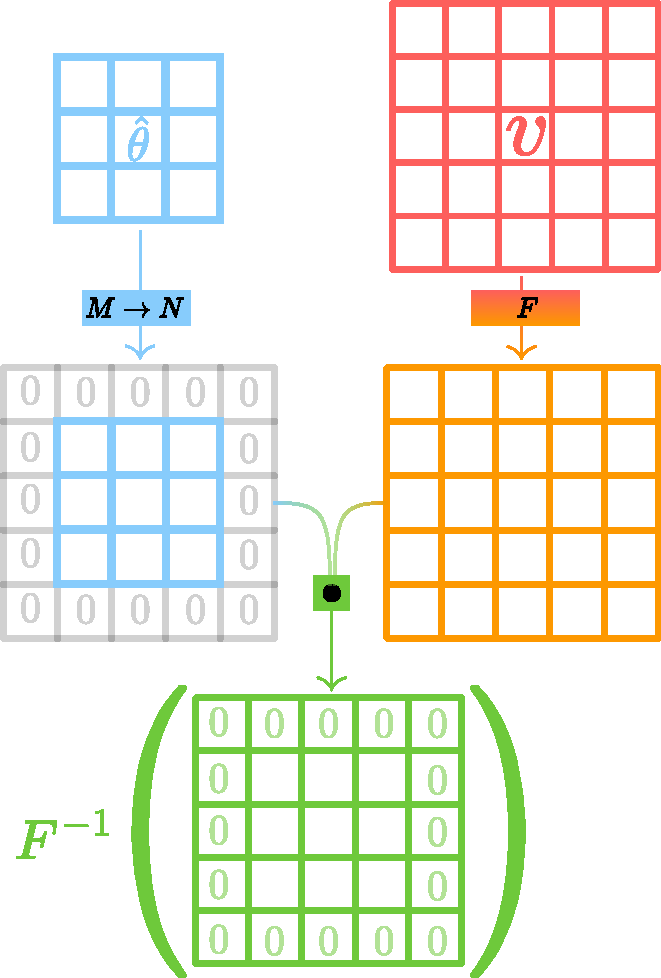
\includegraphics[width=.4\textwidth]{atelier/FNO/trigo.pdf}
\end{wrapfigure}
%
We frequently employ the set $\Inp=[0,1]^{K\times N\times M}$ to represent images. However, from a modeling point of view it is more natural to assume that images are functions $\img:\domain\to[0,1]^K$ where $\domain\subset\R^2$ is some domain. In this sense, the space $\Inp$ only constitutes a discretization of the space of all functions from $\domain$ to $[0,1]^K$. The number of pixels, i.e. $N\cdot M$, relates to the \emph{resolution} of the image, where a higher number of pixels yields a higher resolution. In this sense the resolution is merely an artifact of the restriction to finite dimensions in computer vision and not relevant for the classification. Therefore, one wants to obtain a resolution-independent classifier, which we study in the following.
%
\paragraph{Images, Resolution and Scale}
%
%
For the continuum domain we consider the $d$-dimensional torus $\domain = \mathbb{R}^d / \mathbb{Z}^d$. An image is a function 
%
\begin{align*}
\img:\domain\to[0,1]^K
\end{align*}
%
where $K\in\N$ denotes the number of color channels, see \cite{gonzales1987digital}. In order to represent images on a computer we discretize the domain $\domain$, via a regular grid $\domain_N = \{x_0,\ldots,x_N\}$ indexed by the set
%
\begin{align*}
\mathcal{J}_N := \{0,\ldots, N-1\}^d
\end{align*}
%
with grid points $x_j = j/(N-1)$, see e.g. \cite{kabri2022FNO, kovachki2021universal}. For simplicity we assume an equal number of discretization points in each dimension. Therefore, $N^d$ is the resolution of an image discretized w.r.t. $\mathcal{J}_N$. 

It is important to notice the differences to the concept of \emph{scale}. A change in scale would be a change in the original image domain, for example by zooming in on a certain area. For our image classification examples, we usually assume that the image $\img$ contain a certain entity to be classified. The scale roughly describes how \enquote{big} the entity is, or what percentage of the image it fills. We assume that the scale is fixed. Therefore, changing $N$ directly influences the resolution of discretization.

\paragraph{How do Neural Networks react to Resolution Changes?} In many machine learning application one assumes a fixed input size and therefore a fixed resolution, assuming the same scale throughout the data. Formally, networks are defined as mappings $\net_\param:\R^{K\times N\times N}\to\Delta^C$, i.e. they only accept inputs for the fixed resolution $N$. In order to understand how this constraint can be weakened, we need to consider the concrete structure of our networks, which was similarly done in \cite{kovachki2021universal, kabri2022FNO}. The architectures we consider are feed-forward networks of the form
%
\begin{align*}
\net_\param = \Phi^{\text{class}} \circ \mathcal{S}\circ \Phi^{\text{feature}}
\end{align*}
%
where 
%
\begin{itemize}
\item $\Phi^{\text{feature}}$ is the so-called feature extractor, which should be applicable independently from the input dimension,
\item $\mathcal{S}$ is a function that maps inputs of any size to a fixed output dimension $\R^s$,
\item $\Phi^{\text{class}}:\R^s\to\Delta^C$ denotes the classification layer.
\end{itemize}
%
%
%
The feature extractor usually consists of convolutional layers. As in \cite[Ch. 2]{kabri2022FNO} we consider the discrete convolution of two discretized images $\img_N, \imgg_N$ defined as 
%
\begin{align*}
(\img_N\ast \imgg_N)(x_j) := \sum_{k\in \mathcal{J}_N} \img_N(x_k)\cdot \imgg_N(x_{j-k})
\end{align*}
%
where for negative indices $j-k$ we set $x_{j-k} := x_{j-k+N}$. This assumes that both $\img_N, \imgg_N$ live on the same discretization $\mathcal{J}_N$. Modeling spatial locality---and therefore a small support of the kernel---one usually chooses $M$ much smaller than the resolution. See e.g. the study in \cite{hubel1962receptive} which explores a similar methodology for the visual cortex of cats. In order to account for this dimension mismatch we consider so-called \emph{spatial zero-padding} for kernels $\param\in\R^{\mathcal{J}_M}$
%
\begin{align*}
\param^{M \rightarrow N}_k = 
\begin{cases}
\param_k & \text{for } k \in \mathcal{J}_N \cap \mathcal{J}_M,\\
0 & \text{for } k \in \mathcal{J}_N \backslash \mathcal{J}_M.
\end{cases}
\end{align*}
%
Using this method, one can define the convolution for inputs $u_N$ of arbitrary input resolution $N$ via
%
\begin{align*}
C(\param)(u_N)= \param^{M \rightarrow N} \ast u_N.
\end{align*}
%
In \cite{kabri2023resolution} we refer to this as the \emph{spatial implementation} of convolution. Up to the behavior on the boundary this is in fact the standard implementation in most libraries, especially in \texttt{PyTorch}. Therefore, a feature extractor consisting of convolutional layers can take inputs of variable resolution. In fact, ignoring possible resolution changes within the extractor---i.e. via pooling or strided convolutions---we have that $\Phi^{\text{feature}}(\img_N)\in \R^{\mathcal{J}}_N$ for any $N\in\N$.

The mapping $\mathcal{S}$ can be realized as an adaptive pooling layer, see \cite{paszke2019pytorch}, which ensures a fixed output size. This methodology yields an \emph{discretization invariant architecture}, see \cite{kabri2022FNO, kovachki2021universal, li2020fourier}, which means that from a technical point of view the network is able to produce outputs for inputs with arbitrary discretization. However, we are actually interested in \emph{discretization invariant functionality} (see \cite{kabri2022FNO, kovachki2021universal, li2020fourier}), which also requires that the output is the same over different resolutions.
%
\paragraph{Input Interpolation}
%
%
The technical possibility to handle different input sizes as described above, usually does not perform well in practice. This is due to the fact that in the standard spatial implementation of convolution the support of the kernel changes with varying input dimension, for which it output differs, see \cref{fig:bulbul}. If a network is trained on a fixed input size, the filters are adapted to this size and therefore only create meaningful responses on this size.

A simple attempt to create a network, where not only the architecture, but also the functionality is discretization independent---at least up to a certain degree---is input interpolation. In this case our architecture is modified to
%
\begin{align*}
\tilde \net_\param = \net_\param \circ I
\end{align*}
%
where $I:\bigcup_{M\in\N} \R^{\mathcal{J}_M} \to \R^{\mathcal{J}_N}$ is an interpolation function, that maps inputs of arbitrary sizes to a fixed out discretization $\mathcal{I}_N$. Typical choices here include nearest neighbor, bilinear or bicubic interpolation, see e.g. \cite{gonzales1987digital}. Especially relevant in our case, is so-called \emph{trigonometric interpolation}, where for $\imgg_M\in\R^{\mathcal{J}}$ we define
%
%
\begin{align*}
I^{\text{trigo}}(\imgg_M) := \imgg_M^{M \xrightarrow{\Delta} N} := F^{-1} \left( (Fv)^{M \rightarrow N}\right).
\end{align*}
%
%
\paragraph{Contribution} In \cite{kabri2023resolution} we study the connection between FNOs and CNNs for classification problems. We identify under which assumption the architectures are equivalent (see \cref{lem:FNOconv}), but also where they are not, see \cref{fig:bulbul}. Here, we are especially interested in the multi-resolution case, we show that one layer of an FNO is equivariant with respect to trigonometric interpolation, \cref{cor:FNOequi}. This is also underlined by numerical experiments, where we compare the FNO implementation to interpolation methods and a naive CNN implementation. Furthermore, we show that training equivalent CNN and FNO layers lead to different results, i.e., while they have the same forward pass, the gradients w.r.t. their parameters might differ, \cref{lem:FNOGrad}. Furthermore, we show continuity and Fréchet-differentiability of abstract neural layers as operators between $L^p$ spaces, see \cref{sec:FNOAna}. Finally we conduct numerical experiments supporting our theoretical findings \cref{sec:FNONum}.
%
%

%
%
\subsection{Fourier Neural Operators}
%
%
We want to obtain neural networks whose output does not depend on the discretization of an image $\img:\domain\to\R^K$. This raises the question whether it is possible to find a formulation that allows us to work in the infinite dimensional setting. In \cite{kovachki2021neural} this issue was addressed in the setting of parametric PDEs for which the authors introduced the concept of \emph{neural operators}. One layer of a neural operator is given as a mapping $\mathcal{G}:  L^p(\domain) \rightarrow L^q(\domain)$
%
\begin{align}\label{eq:layerdef}
\mathcal{G}(u)(x) = \sigma\left(\Psi(u)(x)\right) \qquad \text{for a.e. } x \in \domain,
\end{align}
%
with the affine linear part given by
%
\begin{align}\label{eq:linearpart}
\Psi(u) = W u + \mathcal{K}u + b,
\end{align}
%
where
%
\begin{itemize}
\item $\mathcal{K}: u \mapsto \int_{\domain} \kappa(\cdot, y)\, u(y)\,dy$ is a kernel integral operator with kernel $\kappa: \domain \times \domain \rightarrow \R$,
\item $W \in \R$ models a residual component,
\item and $b: \domain \rightarrow \R$ models a bias.
\end{itemize}
%
%
By a slight abuse of notation, the activation function $\sigma:\R\to\R$ acts as a \Nem operator
%
\begin{align}\label{eq:nemytskii}%
\sigma: v \mapsto \sigma(v(\cdot)),
\end{align}
%
see e.g. \cite{tröltzsch}.

In \cref{sec:FNOAna} we analyze continuity and differentiablility of a layer in this abstract form. However, the most relevant case for us, is when $\mathcal{K}$ is a convolution operator, i.e. $\kappa(x,y)=\kappa(x-y)$ is a translation invariant kernel. In this special case $\mathcal{G}$ is then known as layer of a \emph{Fourier Neural Operator} (FNO) as introduced in \cite{li2020fourier}, by parameterizing the kernel via its Fourier coefficients $\hat{\param}_k\in\C$
%
\begin{align}\label{eq:fnokernel}
\kappa_{\hat{\theta}}(x) = \sum_{k \in \mathcal{I}} \hat{\theta}_k\, b_k(x),
\end{align}
%
where $b_k(x) = \exp{(2\pi i\, kx)}$ denote the Fourier basis functions. In practice we assume that $\kappa_{\hat\param}$ only has a finite amount of non-zero Fourier coefficients, in fact we choose the set $\mathcal{I}_N := \lbrace -\lceil (N-1)/2\rceil, \ldots,0, \ldots\,, \lfloor (N-1)/2 \rfloor\rbrace^d$ as the index set, as done in \cite{li2020fourier}. Employing this set with odd $N\in\N$, we can easily enforce Hermitian symmetry $\hat{\theta}_k = \overline{\hat{\theta}_{-k}}$, which ensures that $\mathcal{K}_{\hat\param}$ outputs real-valued functions. For now we assume an odd number here and deal with the even case later. We note that assuming a finite number $N$ of Fourier coefficients is completely independent from the input discretization, which is the main advantage of FNOs.
%
%
\paragraph{How to Perform Convolutions with FNOs?}
%
%
In \cite{kabri2023resolution} we consider the discrete Fourier transform and its inverse
%
\begin{align*}
\left(Fv\right)_k &= \frac{1}{\lambda} \sum_{j \in \mathcal{J}_N} v_j\, e^{-2\pi i \, \left\langle k, \frac{j}{N}\right\rangle},  k \in \mathcal{I}_N,\\
%
\left(F^{-1}\hat{v}\right)_j &= \frac{\lambda}{|\mathcal{J}_N|}\sum_{k \in \mathcal{I}_N} \hat{v}_k\, e^{2\pi i \, \left\langle k, \frac{j}{N}\right\rangle} j \in \mathcal{J}_N,
\end{align*}
%
with a normalization constant $\lambda \in \{1, \sqrt{|\mathcal{J}_N|}, |\mathcal{J}_N|\}$. We only consider parameters $\hat\param\in \Csym^{\mathcal{I}_N} := F(\R^{\mathcal{J}_N})$ for which can employ the convolution theorem (see e.g. \cite{grafakos}) to define
%
\begin{align}\label{eq:discfno}
K(\hat{\theta})(v) = F^{-1}\left(\hat{\theta} \cdot Fv\right) \qquad \text{for }v \in \R^{\mathcal{J}_N}
\end{align}
%
which is referred to as the FNO- or spectral-implementation of convolution.
%
%
\paragraph{How do FNOs React to Resolution Changes?}
%
We already mentioned that the number of Fourier coefficients of $\hat\param\in\Csym^{\mathcal{I}_M}$ is independent of the input resolution. Nevertheless, the point-wise multiplication in \cref{eq:discfno} is only defined for inputs $\imgg\in\R^{\mathcal{J}_M}$, for which the question arises how FNOs can be adapted to dimension mismatch. Here, we apply a conceptually similar idea, by employing zero-padding. However, the important and major difference is that this zero-padding is performed in the spectral domain. Assuming that $N>M$ is odd and that $\imgg_N\in\R^{\mathcal{J}_N}$ we define
%
%
\begin{align*}
\hat{\theta}^{M \rightarrow N}_k = \begin{cases}
\hat{\theta}_k & \text{for } k \in \mathcal{I}_N \cap \mathcal{I}_M,\\
0 & \text{for } k \in \mathcal{I}_N \backslash \mathcal{I}_M,
\end{cases}
\end{align*}
%
%
and the spectral implementation of convolution as
%
%
\begin{equation*}
   K(\hat{\theta})(\imgg_N) := K(\hat{\theta}^{M \rightarrow N})(\imgg_N).
\end{equation*}
%
%
\paragraph{What Is The Difference Between Standard and FNO Implementation?}
%
%
The difference between the spectral and spatial implementation is best explained with \cite[Fig. 1]{kabri2023resolution}, which we repeat in \cref{fig:bulbul} for convenience.
%
%
\begin{figure}[t]
\begin{minipage}[t]{\textwidth}
%\fbox{%
\begin{minipage}{\textwidth}
\begin{minipage}{0.01\textwidth}%
\rotatebox{90}{%
	\scriptsize%
	higher resolution \phantom{------------} 
	original \phantom{-------------} 
	lower resolution\phantom{--}}
\end{minipage}%
\hfill%
\begin{minipage}{0.95\textwidth}
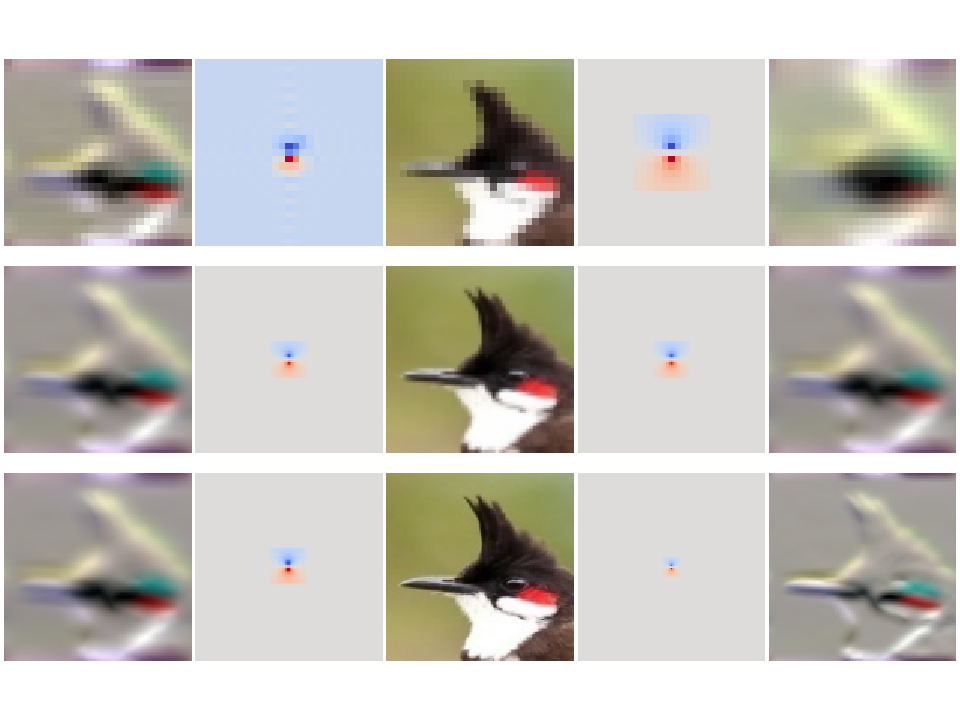
\includegraphics[width=\textwidth, trim= 0cm 1cm 0cm 1cm, clip]{atelier/FNO/res-conv-sobel.pdf}%
\end{minipage}%
\hfill%
\begin{minipage}{0.01\textwidth}
\phantom{-}
\end{minipage}
\end{minipage}
%}%
\hfill%
%
%
\begin{minipage}[t]{.5\textwidth}%
\begin{tikzpicture}[]
\node [
draw=none,
single arrow,
right color=white,
left color=fourierblue,
text=black,
single arrow head extend=0.2cm,
minimum height=\textwidth-5pt,
minimum width=.5cm,
single arrow tip angle=70,
shape border rotate=180
]{\scriptsize Convolution with 
\textbf{spectral} zero-padding};
\end{tikzpicture}\hfill%
%
\end{minipage}%
%
\begin{minipage}[t]{.5\textwidth}%
\hfill%
\begin{tikzpicture}[]
\node [
draw=none,
single arrow,
right color=fourierblue,
left color=white,
text=black,
single arrow head extend=0.2cm,
minimum height=\textwidth-5pt,
minimum width=.5cm,
single arrow tip angle=70,
shape border rotate=0
]{\scriptsize \phantom{-}Convolution with 
\textbf{spatial} zero-padding};
\end{tikzpicture}%
\end{minipage}%
\end{minipage}%
\caption[Effects of applying convolutional filters with different resolutions]{%
The image is taken from \cite[Fig. 1]{kabri2022FNO}---depicting a red whiskered bulbul taken from the Birds500 dataset \cite{pio450}---and visualize the different effects of spectral and spatial zero-padding.}
\label{fig:bulbul}
\end{figure}
%
%
We are given a kernel $\param\in\R^{\mathcal{J}_M}$, its unnormalized Fourier transform $\hat\param = \lambda F(\param)$ and an input $\imgg_N\in \R^{\mathcal{J}_N}$. If $M=N$, i.e. all dimension match, we observe that spectral and spatial implementation are equivalent, see the middle row of \cref{fig:bulbul}. However, if we consider higher resolution variant of the image with $N>M$, spatial zero-padding results in the kernel being localized in space and therefore the effect of convolving it with $\imgg_N$ changes. On the other hand for the spectral implementation we observe an equivariant behaviour. The resolution of the output changes but qualitatively the effect of the filter stay the same.
%
%
\paragraph{Connection to Interpolation}
%
As hinted in \cref{fig:bulbul}, when changing the resolution, the spectral implementation of convolution can be interpreted as a standard convolution with an interpolated kernel. In fact we observe that for $\param\in\R^{\mathcal{J}_M}, \hat\param=\lambda\, F(\param)$ and $\imgg_N\in\R^{\mathcal{J}_N}$ we have that
%
\begin{align*}
\CF(\hat\param)(\imgg_N) &= 
K(\hat{\param}^{M \rightarrow N})(\imgg_N) = 
F^{-1}\left(\hat{\theta}^{M \rightarrow N} \cdot Fv_N\right)\\ 
&= 
%
F^{-1}\left(F\, F^{-1}\hat{\theta}^{M \rightarrow N} \cdot Fv_N\right)\\
%
&=
F^{-1}\left(F \param^{M \xrightarrow{\Delta} N}  \cdot Fv_N \right)
%
=
%
\param^{M \xrightarrow{\Delta} N} \ast \imgg_N\\
%
&= 
C(\param^{M \xrightarrow{\Delta} N})(\imgg_N).
\end{align*}
%
%
Therefore, applying one FNO layer is equivalent to trigonometric interpolation of the kernel.
%
%
\paragraph{Adaption to Even Dimensions}
%
%
Zero-padding of the spectral coefficients only fulfills Hermitian symmetry in the case where $M,N$ are odd. In order ot adapt this to the even case, we employ so-called Nyquist splitting, see \cite{trigo19}. In all our experiments the implementation carefully employs this method, which ensures that the output of the spectral convolution is real valued.
%
%
\subsection{Analytical Results for FNOs}\label{sec:FNOAna}
%
%
In this section, we comment on the theoretical findings in \cite{kabri2023resolution}. We first consider the abstract neural layer as in \cref{eq:layerdef} for which we show continuity and Fréchet-differentiability.
%
%
\paragraph{Continuity of Neural Layers} The results for neural layers in \cite{kabri2023resolution} mostly fall back to the theory of \Nem{} operators, see e.g. \cite{tröltzsch, ambrosetti}. In order to show that the layer $\mathcal{G}$ is a well defined mapping from $L^p$ to $L^q$ one first needs to identify an exponent $r\in [1,\infty]$ such that the affine part is a mapping $\Psi:L^p\to L^r$. For example if $\kappa\in L^s$ with $1/r + 1 = 1/p + 1/s$ it follows from Young's convolution inequality that $\mathcal{K}$ maps to $L^r$, see \cite[Th. 1.2.12]{grafakos}. If then $W=0$ and $b\in L^r$ we know that $\Psi$ maps to $L^r$.

To ensure that the \Nem{} operator defines a mapping $\sigma:L^r\to L^q$ one needs to assume a growth condition on $\sigma:\R\to\R$, see \cite[Eq. 4]{kabri2023resolution} and originally \cite{tröltzsch}. Under these assumptions, we have the following result. The prove is trivial and the main content is buried in the assumptions, however it still summarizes the situation in a convenient way. Concrete examples fulfilling these assumptions are given in \cite{kabri2023resolution} borrowing concepts from \cite{ambrosetti, tröltzsch}. The most important activation function that is valid in this setting is the ReLU function
%
\begin{align*}
\relu(x) = \max\{x, 0\}.
\end{align*}
%
%
\begin{proposition}{\cite[Prop. 1]{kabri2023resolution}}{}
	For $1 \leq p, q \leq \infty$ let $\mathcal{L}$ be an operator layer given by \eqref{eq:layerdef} with an activation function $\sigma: \R \rightarrow \R$.
	If there exists $r \geq 1$ such that
	\begin{enumerate}[label=(\roman*)]
		\item the affine part defines a mapping $\Psi: L^p(\domain) \rightarrow L^r(\domain)$,
		\item the activation function $\sigma$ generates a Nemytskii operator $\sigma: L^r(\domain) \rightarrow L^q(\domain)$,
	\end{enumerate}
	%
	then it holds that
	%\begin{align*}
	$
	\mathcal{L}: L^p(\domain) \rightarrow L^q(\domain).
	$
	%\end{align*}
	If additionally $\Psi$ is a continuous operator on the specified spaces and the function $\sigma$ is continuous, or uniformly continuous in the case $q=\infty$, the operator $\mathcal{L}: L^p(\domain) \rightarrow L^q(\domain)$ is also continuous.
\end{proposition}
%
%
\paragraph{Differentiability of Neural Layers}
%
%
We furthermore consider Fréchet differentiability of a neural layer w.r.t. to the input variable. This can also be transferred to differentiability w.r.t. the parameters as we provide in \cite[Ex. 4]{kabri2023resolution}. Conceptually the main result we repeat here is similar to the one on continuity of the last paragraph. Namely, we put certain assumptions on the affine part and the activation function $\sigma:\R\to\R$ that allow us to employ the classical theory on \Nem{} operators. The major difference is that we also need to assume differentiability of the activation function, were we also assume a growth condition on the derivative. The ReLU function can therefore not be chosen in this setting, however the smooth approximation called GELU (\cite{hen16})
%
\begin{align*}
\operatorname{GELU}(x) := x\, \Phi(x)
\end{align*}
%
where $\Phi$ is the CDF of the standard normal distribution, can be employed.
%
%
\begin{proposition}{\cite[Prop. 2]{kabri2023resolution}}{}
	For $1 \leq p, q \leq \infty$, let $\mathcal{L}$ be an operator layer given by \eqref{eq:layerdef} with affine part $\Psi$ as in \eqref{eq:linearpart}. If there exists $r>q$, or $r = q = \infty$ such that
	\begin{enumerate}[label=(\roman*)]
		\item the affine part is a continuous operator $\Psi: L^p(\domain) \rightarrow L^r(\domain)$,
		\item the activation function $\sigma: \R \rightarrow \R$ is continuously differentiable
		\item and the derivative of the activation function generates a Nemytskii operator $\sigma': L^r(\domain) \rightarrow \left[L^r(\domain) \rightarrow L^{s}(\Omega) \right]$ with $s = {rq}/{(r-q)}$,
	\end{enumerate}
	then it holds that $\mathcal{L}:  L^p(\domain) \rightarrow L^q(\domain)$ is Fréchet-differentiable in any $v \in L^p(\domain)$ with Fréchet-derivative $D\mathcal{L}(v): L^p(\domain) \rightarrow L^q(\Omega)$
	\begin{align*}
		D\mathcal{L}(v)(h) = \sigma'(\Psi(v))\cdot\Tilde{\Psi}(h),
	\end{align*}
	where $\Tilde{\Psi}$ denotes the linear part of $\Psi$, i.e., $\Tilde{\Psi} = \Psi - b$.
\end{proposition}
%
%
\paragraph{Convertibility Between FNOs and CNNs}
%
%
The following lemma formalizes the intuition that FNOs and CNNs are equivalent in certain settings. Given inputs of a fixed discretization $\mathcal{J}_N$ and parameters $\param\in\R^{\mathcal{J}_M}$ the standard convolution implementation is equivalent to the spectral one w.r.t. the parameters $\hat\param = \lambda\, F(\param^{M\to N})$. The subtle but important point here, is that the number of spectral parameters needs to be equal to the input size in order to achieve equivalence. In \cite[Fig.3]{kabri2023resolution} we observe numerically that the number of used spectral coefficients actually needs to match the input size in order to achieve equivalence.
%
%
\begin{lemma}{\cite[Lem. 3]{kabri2023resolution}}{lem:FNOconv}
	Let $M \leq N$ both be odd and let $T: \R^{J_N} \rightarrow \mathbb{C}^{I_N}$ be defined for $\theta \in \R^{J_N}$ as
	$T(\theta) = \lambda \, F(\theta)$.
	For any $\theta \in \R^{J_M}$ and $v \in \R^{J_N}$ it holds true that
	\begin{align*}
		C(\theta)(v) = K(T(\theta^{M\rightarrow N}))(v)
	\end{align*}
	and for any $\hat{\theta} \in \mathbb{C}^{I_M}_{\text{sym}}$ and $v \in \R^{J_N}$ it holds true that
	\begin{align*}
		K(\hat{\theta})(v) = C(T^{-1}(\hat{\theta}^{M\rightarrow N}))(v).
	\end{align*}
\end{lemma}
%
%
\noindent%
From this and from \cite[Fig. 3]{kabri2023resolution} we obtain the negative result that in order to convert a CNN to a FNO we need a large number of spectral parameters. This also connected to the fact that spatial locality can usually only expressed using more spectral coefficients. Therefore, one might think that FNOs are infeasible due to memory requirements. However, it turns out that directly optimizing over the spectral parameters leads to a comparable performance, already for a low number of Fourier coefficients. This is reported in the blue curve in \cite[Fig. 3]{kabri2023resolution}. This hints, that while the forward pass can be equivalent, computing the gradient w.r.t. their parameters is not. This is formalized in the following lemma.
%
%
\begin{lemma}{\cite[Lem. 4]{kabri2023resolution}}{lem:FNOGrad}
For odd $N \in \mathbb{N}$ and $v, \theta \in \R^{J_N}$ and $\hat{\theta} = T(\theta)$ it holds true that
\begin{align*}
	\nabla_{\hat{\theta}} K(\hat{\theta})(v) = \frac{1}{|J_N|}\; T \left( \vphantom{\hat{\theta}} \nabla_{\theta}C(\theta)(v) \right). 
\end{align*}
\end{lemma}
%
%
\paragraph{Interpolation Equivariance}
%
%
The last result considers the main motivation for the topic. Namely, the resolution in-variance of an FNO layer. However, here we can not allow an arbitrary resizing operation. Since it is most natural to our approach, we can show equivariance w.r.t. trigonometric interpolation of the input.
%
%
\begin{corollary}{}{cor:FNOequi}
	For $\hat{\theta} \in \mathbb{C}^{I_M}_{\text{sym}}$, $v \in \R^{J_N}, M \leq N$ it holds true for any $L \geq M$ that
	\begin{align*}
		K(\hat{\theta})(v^{N \xrightarrow{\Delta} L}) = \left( K(\hat{\theta})(v) \right)^{N \xrightarrow{\Delta} L}.
	\end{align*}
\end{corollary}


\subsection{Numerical Results}\label{sec:FNONum}
%
%
\begin{wrapfigure}{r}{.4\textwidth}
\begin{center}
	
\includegraphics[width=.4\textwidth]{atelier/FNO/FNOQR.png}
\end{center}
The code for all the experiments is available at \href{https://github.com/samirak98/FourierImaging}{https://github.com/samirak98/}\\
\href{https://github.com/samirak98/FourierImaging}{FourierImaging}.
\end{wrapfigure}
%
%
In the numerical section of \cite{kabri2023resolution} we study the convertibility of CNNs to FNOs as discussed in \cref{sec:FNOAna} and the resolution invariance of the different proposed approaches. Again we employ---among others---the \texttt{PyTorch} package \cite{paszke2019pytorch}. The experiments are conducted on the FashionMNIST \cite{Han17} and a former version of the BIRDS500 \cite{pio450} dataset. We remark that our implementation carefully treats the case of even kernel or input sizes, via Nyquist splitting. This allows us to apply all the derived results for the odd and also the even case.
%
%
\paragraph{Convertibility and Training Differences} As already described in \cref{sec:FNOAna} the first experiment, displayed in \cite[Fig. 3]{kabri2023resolution}, studies how CNNs can be converted to FNOs. Here, we employ a network with two convolutional layers for feature extraction and a linear classification layer. We train this network---in the spatial implementation---on the FashionMNIST dataset employing varying spatial kernel sizes. Here, we see that for $M=5$ the spatial implementation already has the best performance and adding more parameters does not increase the performance. We then convert a set of spatial parameters to the Fourier formulation, employing again a varying number of spectral coefficients. It turns out that the requirement of \cite[Lem. 3]{kabri2023resolution}, that the number of coefficients must match the input dimension is indeed relevant. We only obtain the full performance of the CNN if we use all spectral parameters. However, the example also visualizes \cite[Lem. 4]{kabri2023resolution}, namely that training a FNO conceptually leads to a different set of parameters. Optimizing over the spectral parameters yields a comparable performance already for a smaller number of coefficients.
%
%
\paragraph{Resolution Invariance}
%
In the second experiment we study the resolution invariance of the three discretization independent architectures we considered, namely the naive CNN adaptation, input interpolation and the FNO implementation. We first train the convolutional architecture as in the previous paragraph on the FashionMNIST dataset, that has an input size of $28\times 28$. We resize the input data via trigonometric and bilienear interpolation---referred to as data sizing---to simulate multi-resolution data. One expects that the classification performance drops when the data is resized to a smaller size, since this step looses information. However, resizing the images to higher resolutions should yield the same performance.

In \cite[Fig. 4]{kabri2023resolution} see that the simple adaption does not perform well both in the lower and the higher resolution setting. Employing input interpolation improves the performance in the lower resolution setting. In the higher resolution regime, we obtain a constant performance which is expected. Finally we see that the FNO---which was converted from the CNN---performs as well as input interpolation, which justifies the resolution independence of this architecture.

In the second experiments we trained a ResNet18 \cite{he2016deep} on a former version of the BIRDS500 dataset, with an input size of $112\times 112$. Concerning the naive adaption and the input interpolation we observe the same behavior as in the previous example. However, the FNO variant performs slightly worse, which is surprising, especially in the higher resolution regime. In \cite{kabri2023resolution} we conclude that this is due the dimension changes within the ResNet architectures. These changes occur due to strided convolutions or pooling operations between the layers. In fact in order to achieve the performance as displayed in \cite[Fig. 4 (b)]{kabri2023resolution} we replaced every striding by a trigonometric interpolation, which fits better into the FNO framework and vastly improves the performance. Therefore, we summarize that architecture intern dimension changes---which are very common in practice---can potentially hinder resolution invariance.